\section{general update}

\begin{frame}
\frametitle{a single, big image}
\vspace{-0.24 cm}
\begin{center}
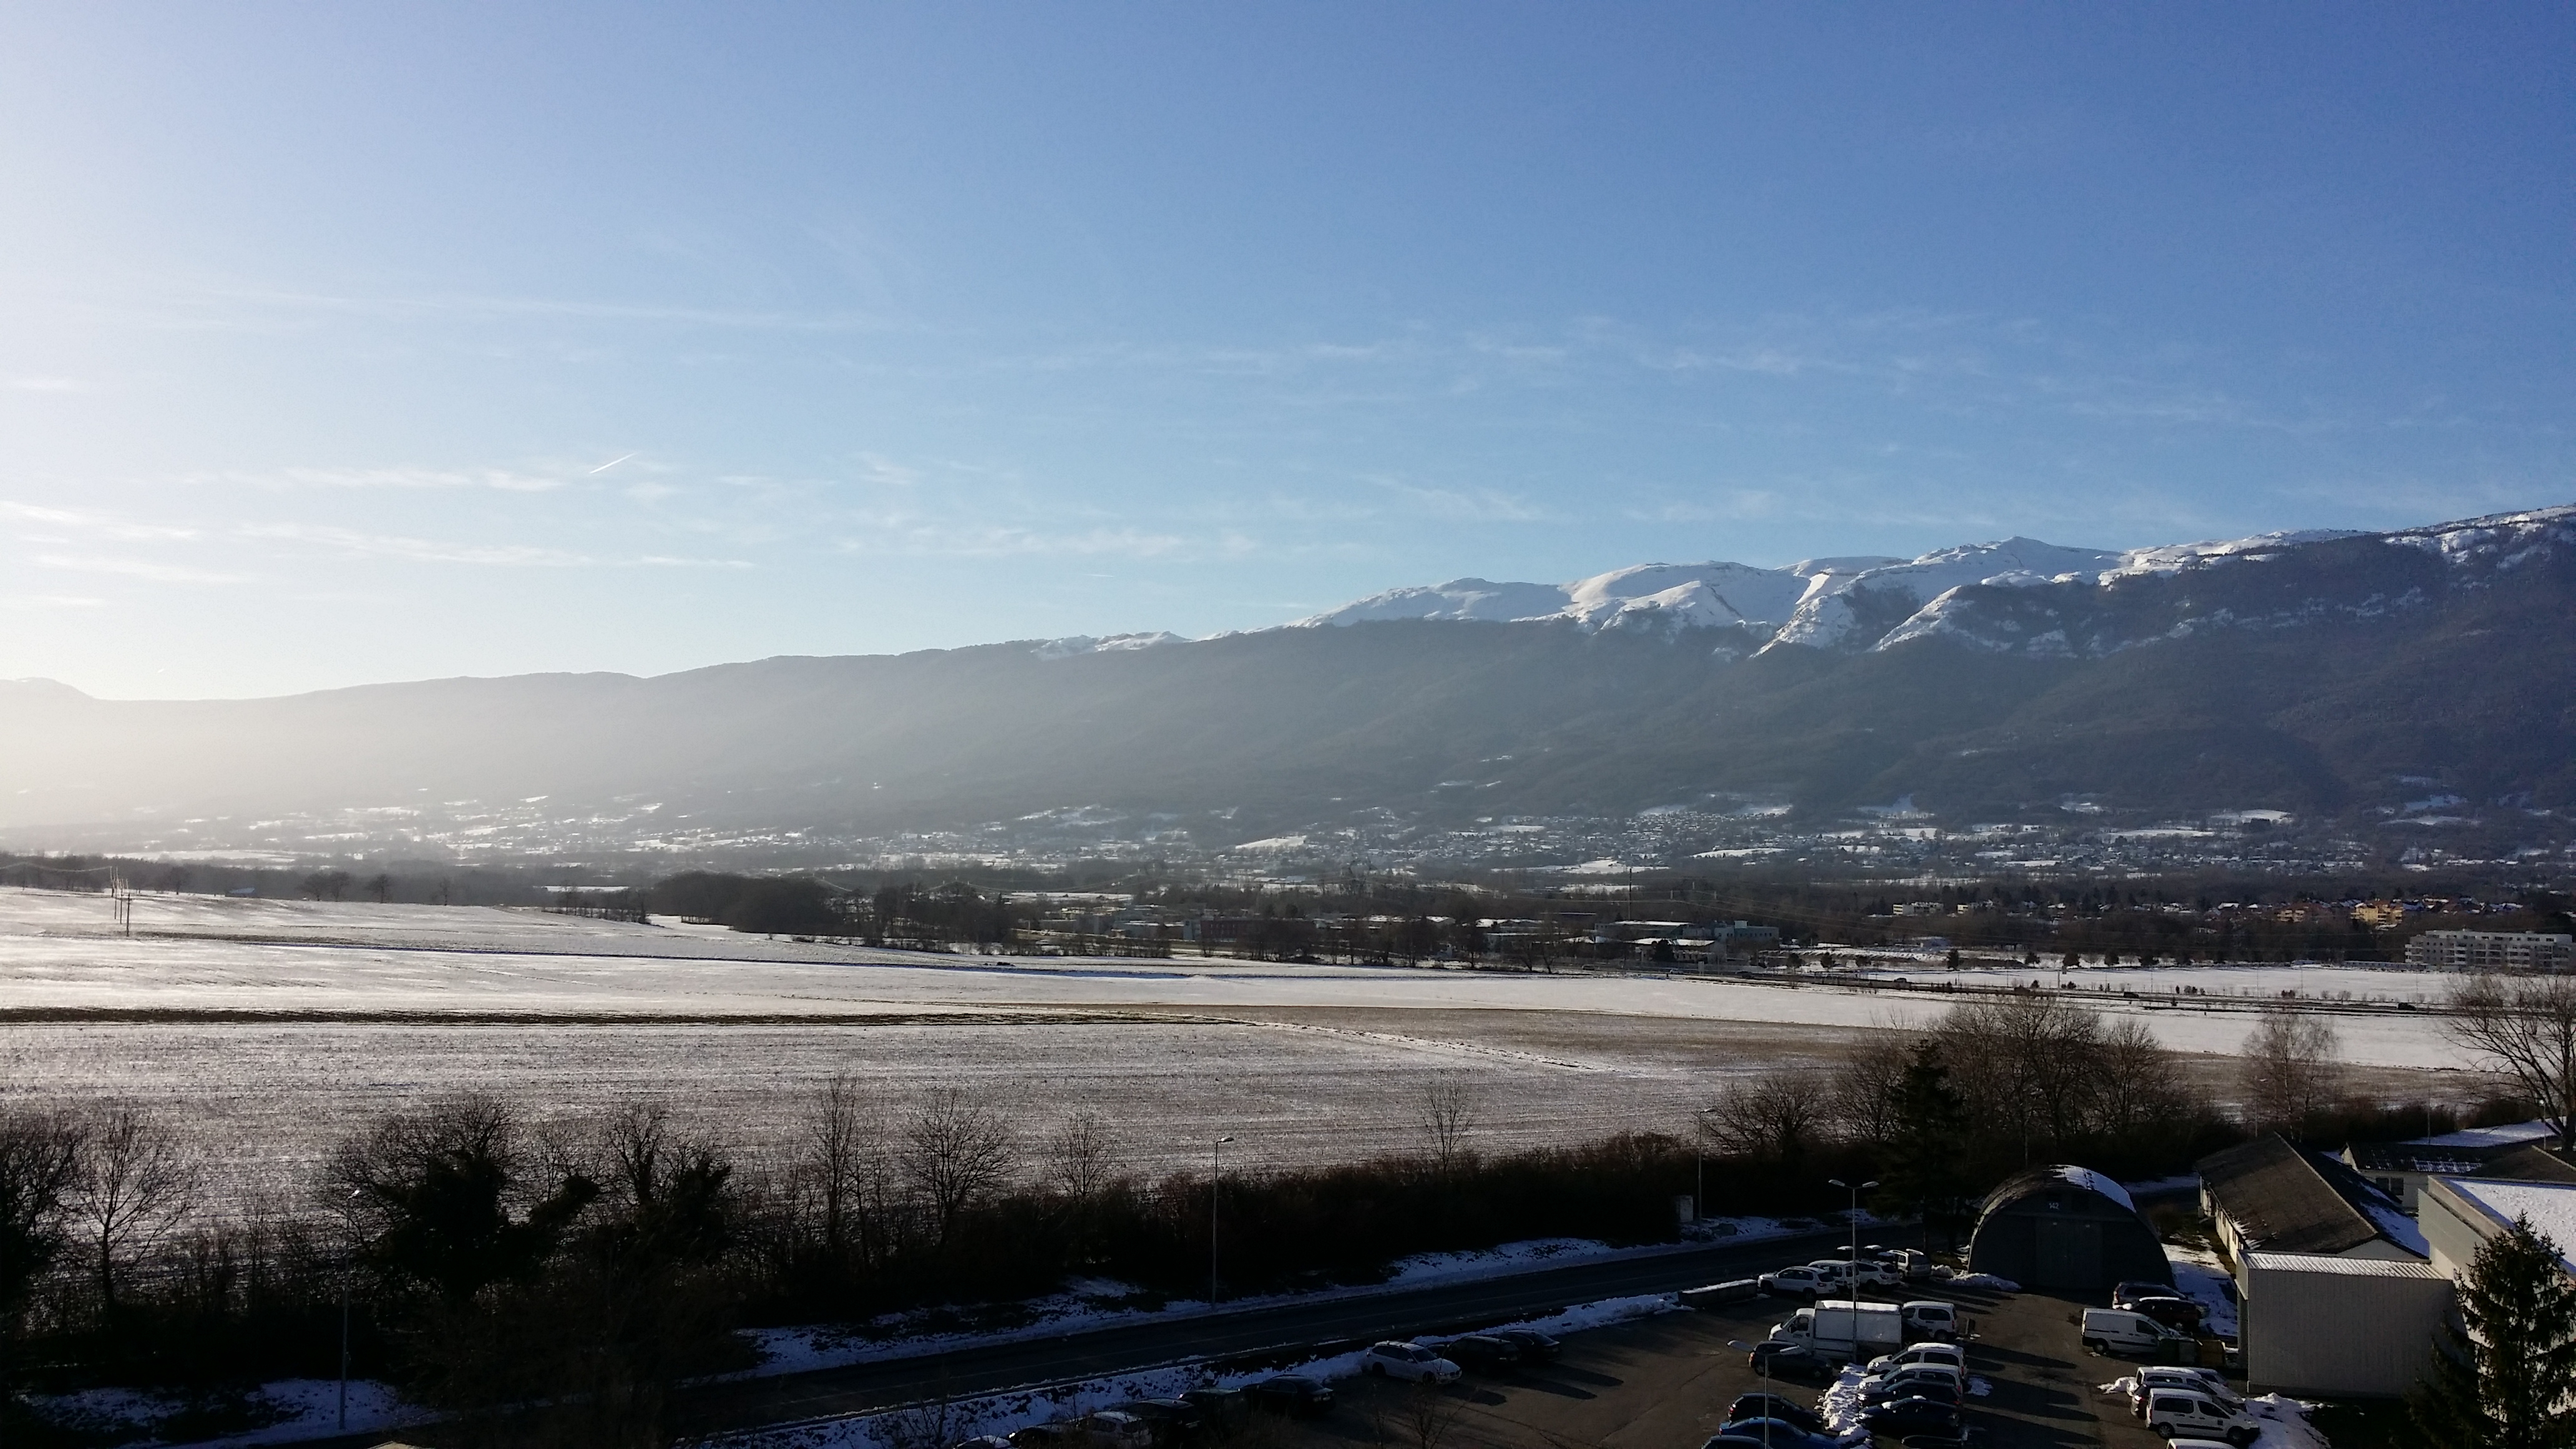
\includegraphics[width=\measureUSpecification]{\directoryImagesA/2015-02-09T161202.jpg}\\
\end{center}
\end{frame}

\begin{frame}
\frametitle{an animated image (compatible with Adobe Reader)}
\vspace{-0.24 cm}
\begin{center}
%\animategraphics[
%    autoplay,
%    loop,
%    width=\measureUSpecification
%]{<frame rate>}{file path and basename}{<first>}{<last>}\\
\animategraphics[
    autoplay,
    loop,
    width=\measureUSpecification
]{30}{\directoryImagesA/pool/pool_}{0}{29}\\
\end{center}
\end{frame}

\begin{frame}
\frametitle{a video (compatible with Okular)}
\vspace{-0.24 cm}
\begin{center}
\movie[
    height=6 cm,
    width=8 cm,
    showcontrols,
    poster
]{
\includegraphics[width=8 cm]{\directoryVideosA/hokeymon.png}}{\directoryVideosA/hokeymon.mp4}
\end{center}
\end{frame}

\begin{frame}
\frametitle{itemized list}
\begin{itemize}
\item item
\item item
    \begin{itemize}
    \item subitem
    \item subitem
        \begin{itemize}
        \item subitem
        \end{itemize}
    \end{itemize}
\item item
\item item
\end{itemize}
\end{frame}

\begin{frame}
\frametitle{enumerate list}
\begin{enumerate}
\item item
\item item
    \begin{enumerate}
    \item subitem
    \item subitem
        \begin{enumerate}
        \item subitem
        \end{enumerate}
    \end{enumerate}
\item item
\item item
\end{enumerate}
\end{frame}

\begin{frame}
\frametitle{description list}
\begin{description}
\item[A] item
\item[B] item
    \begin{description}
    \item[A] subitem
    \item[B] subitem
        \begin{description}
        \item[A] subitem
        \end{description}
    \end{description}
\item[C] item
\item[D] item
\end{description}
\end{frame}

% \checkmark (amsmath)
% \Checkmark
% \CheckmarkBold
% \XSolidBrush

\begin{frame}
\frametitle{description list with checkmarks}
\begin{description}
\item[\Checkmark] item
\item[\Checkmark] item
    \begin{description}
    \item[\Checkmark] subitem
    \item[\textbullet] subitem
        \begin{description}
        \item[\textbullet] subitem
        \end{description}
    \end{description}
\item[\Checkmark] item
\item[\XSolidBrush] item
\end{description}
\end{frame}

\begin{frame}
\frametitle{links}
\begin{itemize}
\item URL: \url{http://info.cern.ch/hypertext/WWW/TheProject.html}
\item hyperlink: \href{http://info.cern.ch/hypertext/WWW/TheProject.html}{TheProject}
\item hyperlink: \href{https://cds.cern.ch/record/1969527}{ATL-COM-PHYS-2014-1471}
\end{itemize}
\end{frame}

\begin{frame}
\frametitle{mathematics}
\begin{itemize}
\item ${H^{+}\to tb}$
\item lepton ${p_{T}}$ and ${\eta}$
\end{itemize}
\end{frame}

\begin{frame}
\frametitle{emoticons}
\begin{itemize}
\item smiley: \smiley
\item frownie: \frownie
\item neutralie: \neutralie
\end{itemize}
\end{frame}

\begin{frame}
\frametitle{centered text}
\begin{center}
some centered text\\\mbox{}\\some more centered text\\\mbox{}\\
\end{center}
\end{frame}

\begin{frame}
\frametitle{blocks}
\begin{block}{block 1}
\begin{itemize}
\item item
\item item
\end{itemize}
\end{block}
\begin{block}{block 2}
\begin{itemize}
\item item
\item item
\end{itemize}
\end{block}
\end{frame}

\begin{frame}
\frametitle{columns (2)}
\begin{columns}
\begin{column}[t]{.5\textwidth}
\justifying
Lorem ipsum dolor sit amet, consectetuer adipiscing elit. Aenean commodo ligula eget dolor. Aenean massa. Cum sociis natoque penatibus et magnis dis parturient montes, nascetur ridiculus mus. Donec quam felis, ultricies nec, pellentesque eu, pretium quis, sem.
\end{column}
\hfill
\begin{column}[t]{.5\textwidth}
\justifying
Nulla consequat massa quis enim. Donec pede justo, fringilla vel, aliquet nec, vulputate eget, arcu. In enim justo, rhoncus ut, imperdiet a, venenatis vitae, justo. Nullam dictum felis eu pede mollis pretium.
\end{column}%
\end{columns}
\end{frame}

\begin{frame}
\frametitle{multiple columns (2)}
\setlength\columnsep{30pt}
\begin{multicols}{2}
\justifying
Lorem ipsum dolor sit amet, consectetuer adipiscing elit. Aenean commodo ligula eget dolor. Aenean massa. Cum sociis natoque penatibus et magnis dis parturient montes, nascetur ridiculus mus. Donec quam felis, ultricies nec, pellentesque eu, pretium quis, sem. Nulla consequat massa quis enim. Donec pede justo, fringilla vel, aliquet nec, vulputate eget, arcu. In enim justo, rhoncus ut, imperdiet a, venenatis vitae, justo. Nullam dictum felis eu pede mollis pretium.
\end{multicols}
\end{frame}

\begin{frame}
\frametitle{multiple columns (4)}
\setlength\columnsep{30pt}
\begin{multicols}{4}
\justifying
Lorem ipsum dolor sit amet, consectetuer adipiscing elit. Aenean commodo ligula eget dolor. Aenean massa. Cum sociis natoque penatibus et magnis dis parturient montes, nascetur ridiculus mus. Donec quam felis, ultricies nec, pellentesque eu, pretium quis, sem. Nulla consequat massa quis enim. Donec pede justo, fringilla vel, aliquet nec, vulputate eget, arcu. In enim justo, rhoncus ut, imperdiet a, venenatis vitae, justo. Nullam dictum felis eu pede mollis pretium.
\end{multicols}
\end{frame}

\begin{frame}
\frametitle{positioning by textblock}
\vspace{-7 cm}
\small
\begin{textblock}{8}(0.25, 2.15) % upper left
\begin{itemize}
\item suppressed with respect to other Higgs modes
\item ${H\to b\bar{b}}$ has the largest branching ratio\\(0.577 for ${m_{H}}$ 125~GeV)
\item irreducible background from ${t\bar{t}b\bar{b}}$
\item other backgrounds: ${t\bar{t}}$ production in association with light quarks (${u}$, ${d}$, ${s}$) or gluon jets\\(called ${t\bar{t}}$ + light), and ${t\bar{t}+c\bar{c}}$
%\item large uncertainties on ${t\bar{t}}$ + HF
\end{itemize}
\end{textblock}
\begin{textblock}{8}(8.75, 2.15) % upper right
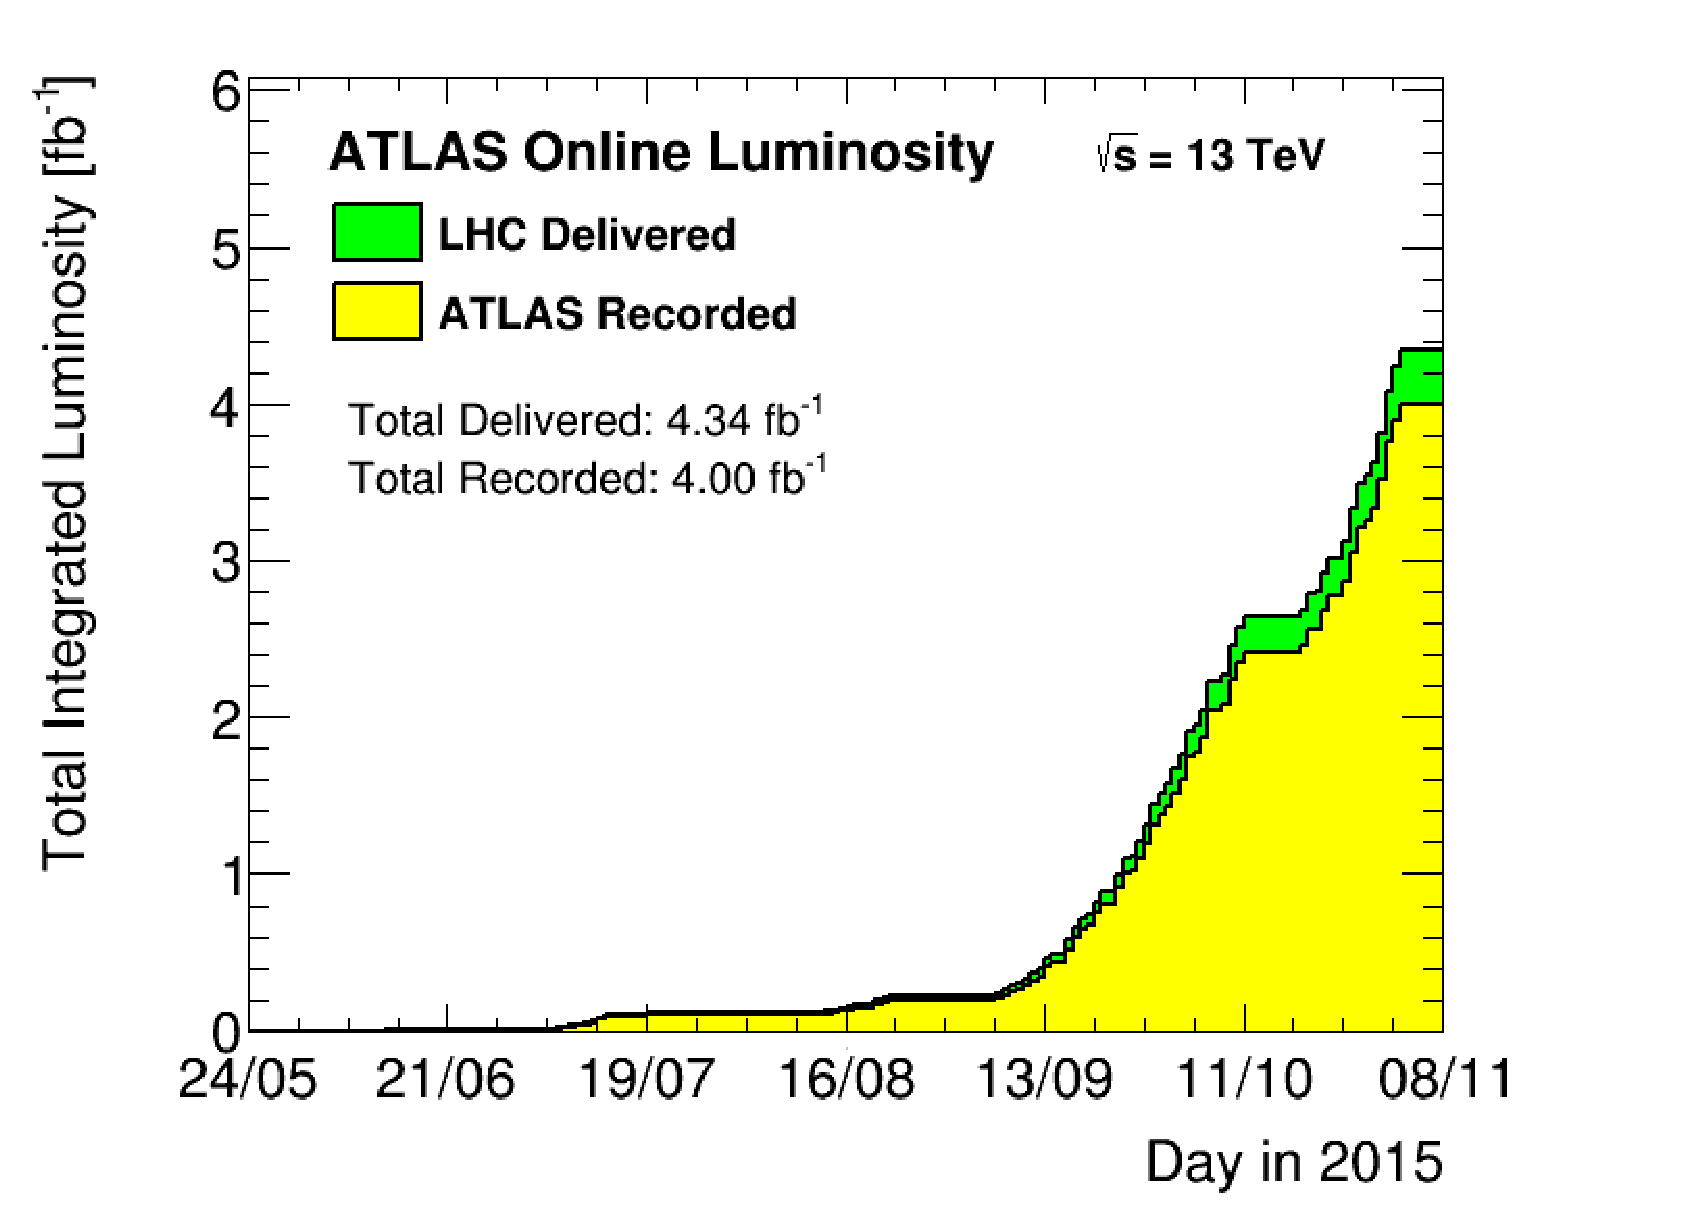
\includegraphics[height=4.5 cm]{\directoryImagesB/sumLumiByDayUrgent}
\end{textblock}
\begin{textblock}{8}(2.75, 10.5) % lower left
\begin{centering}
\begin{tabular}{r|c|c|c|c}
    ${\sqrt{s}}$ (TeV) & 7 & 8 & 13 & 14 \\
    \hline
    ${t\bar{t}H}$ (${m_{H}=125\textrm{ GeV}}$) (pb) & 0.086 & 0.130 & 0.5085 & 0.611 \\
    ${t\bar{t}}$ (pb) & 177 & 253 & 832 & 950 \\
    \hline
    S/${\sqrt{\textrm{B}}}$ & 0.00646 & 0.0082 & 0.0176 & 0.0198 \\
\end{tabular}
\end{centering}
\mbox{}\\
\mbox{}\\
\tiny
7~TeV ${\to}$ 13/14~TeV: ${S/\sqrt{B}}$ changes by factor of ${\simeq}$3
\end{textblock}
%\begin{textblock}{8}(8.25, 8.75) % lower right
%\end{textblock}
\end{frame}

%\begin{frame}[fragile]
%\frametitle{global interpreter lock (GIL) in Python}
%The Python interpreter is not fully thread safe and, so, a GIL is implemented in order to support multithreaded Python programs. Without the GIL, even many simple operations are problematic (e.g. incrementing the reference count of some common object simultaneously in two threads could result in a single increment, rather than the intended two increments).\\
%\mbox{}\\
%rule: Only the thread that has acquired the GIL my operate on Python objects or call API functions.\\
%\mbox{}\\
%The Python interpreter attempts to switch threads regularly (using \pythoninline{set.checkinterval()}) in order to emulate concurrency.
%\end{frame}

%\begin{frame}[fragile]
%\frametitle{a taste of Python multiprocessing: creating a process}
%\begin{python}
%from multiprocessing import Process
%
%def function1(text):
%    print(text)
%
%if __name__ == "__main__":
%    process1 = Process(target = function1, args = ("hello world",))
%    process1.start()
%    process1.join()
%\end{python}
%\end{frame}

\begin{frame}
\frametitle{${8\textrm{ TeV}}$ vs.~${13\textrm{ TeV}}$: cutflow for ${l+\textrm{jets}}$}
\begin{center}
\begin{tabular}{cc}
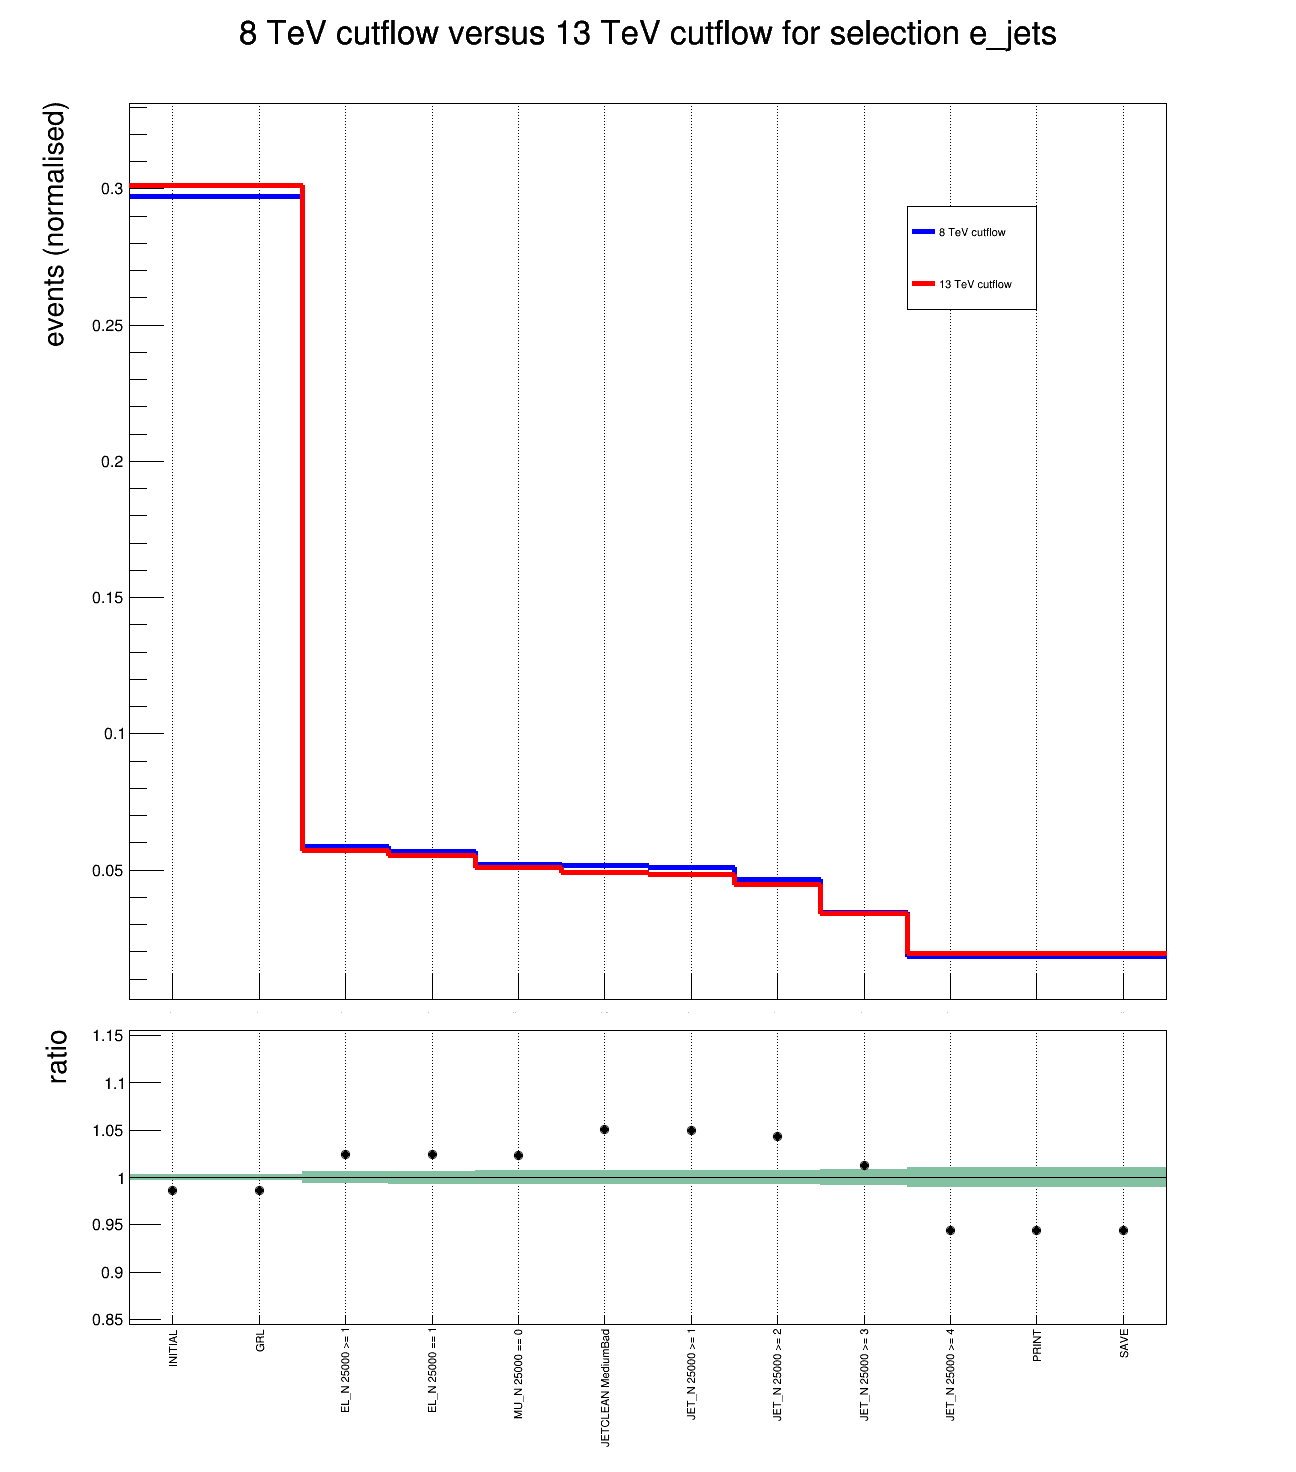
\includegraphics[width=\measureNSpecification]{\directoryImagesB/2015-04-21T0410Z_cutflow_e_jets.png}&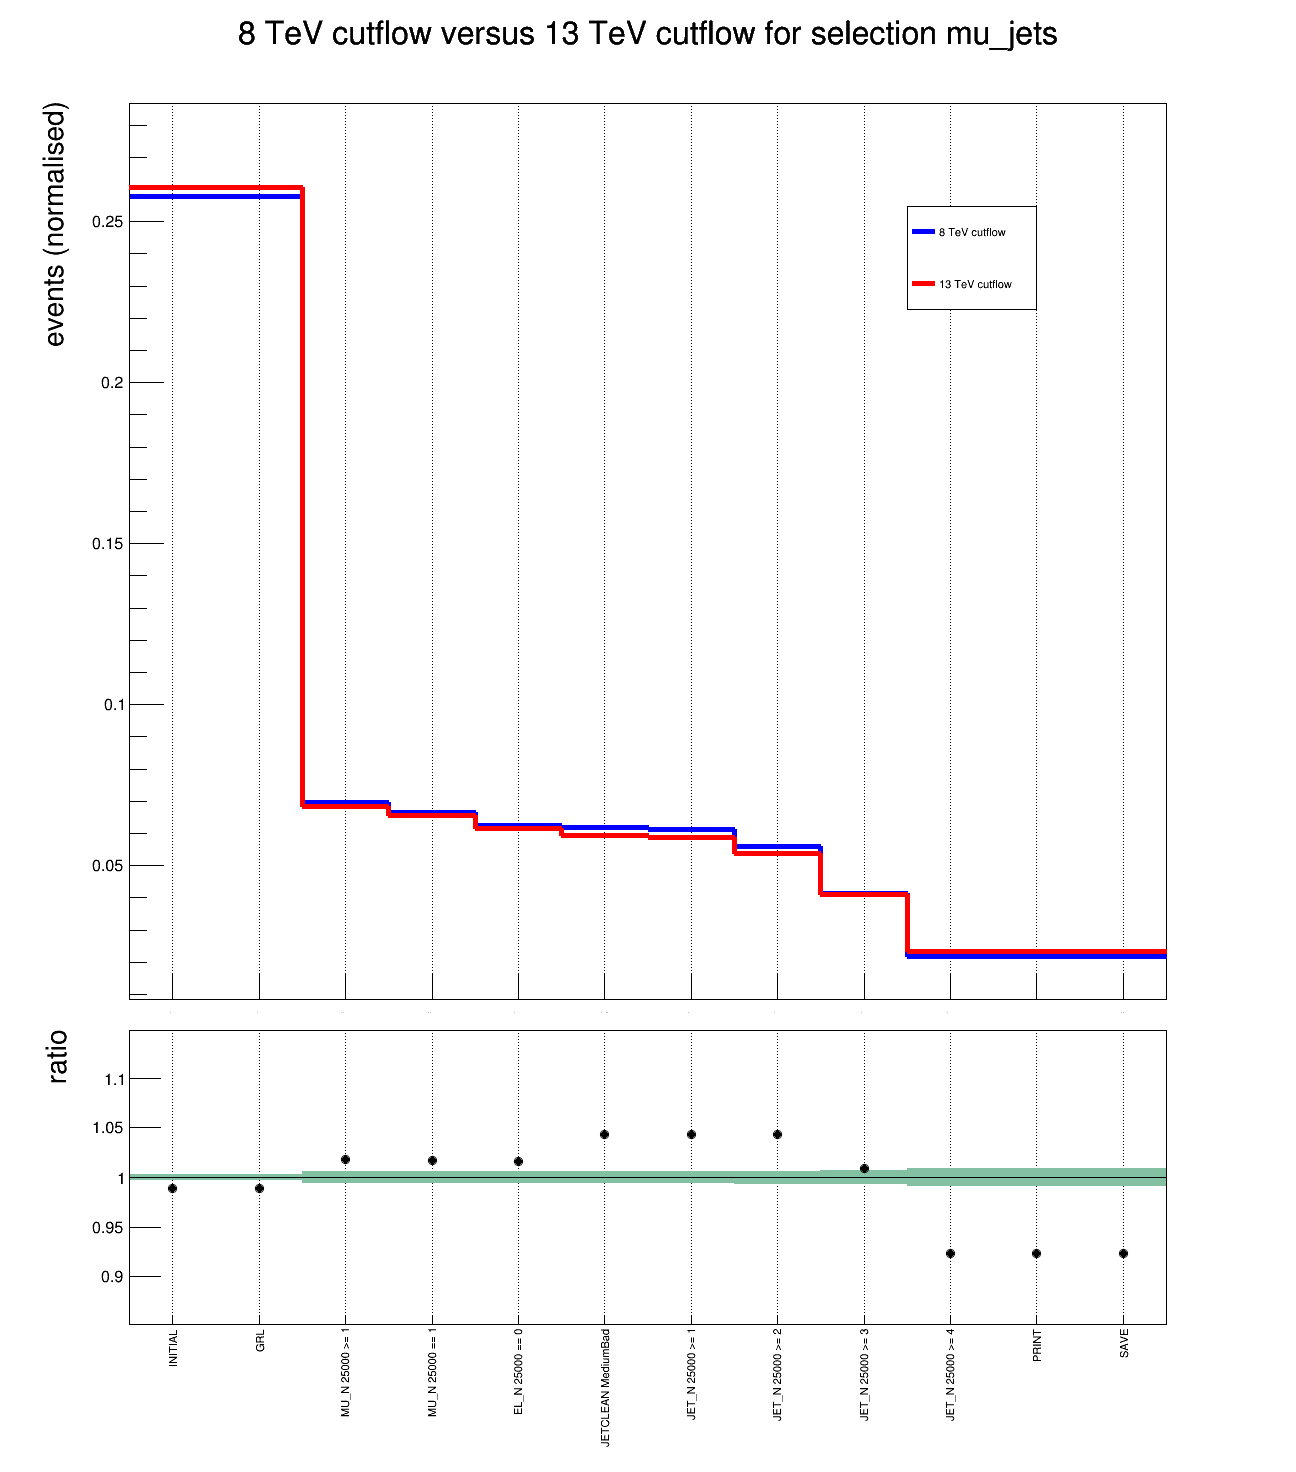
\includegraphics[width=\measureNSpecification]{\directoryImagesB/2015-04-21T0410Z_cutflow_mu_jets.png}\\
\end{tabular}
\end{center}
\end{frame}

\begin{frame}
\frametitle{${8\textrm{ TeV}}$ vs.~${13\textrm{ TeV}}$: cutflow for dilepton}
\begin{center}
\begin{tabular}{ccc}
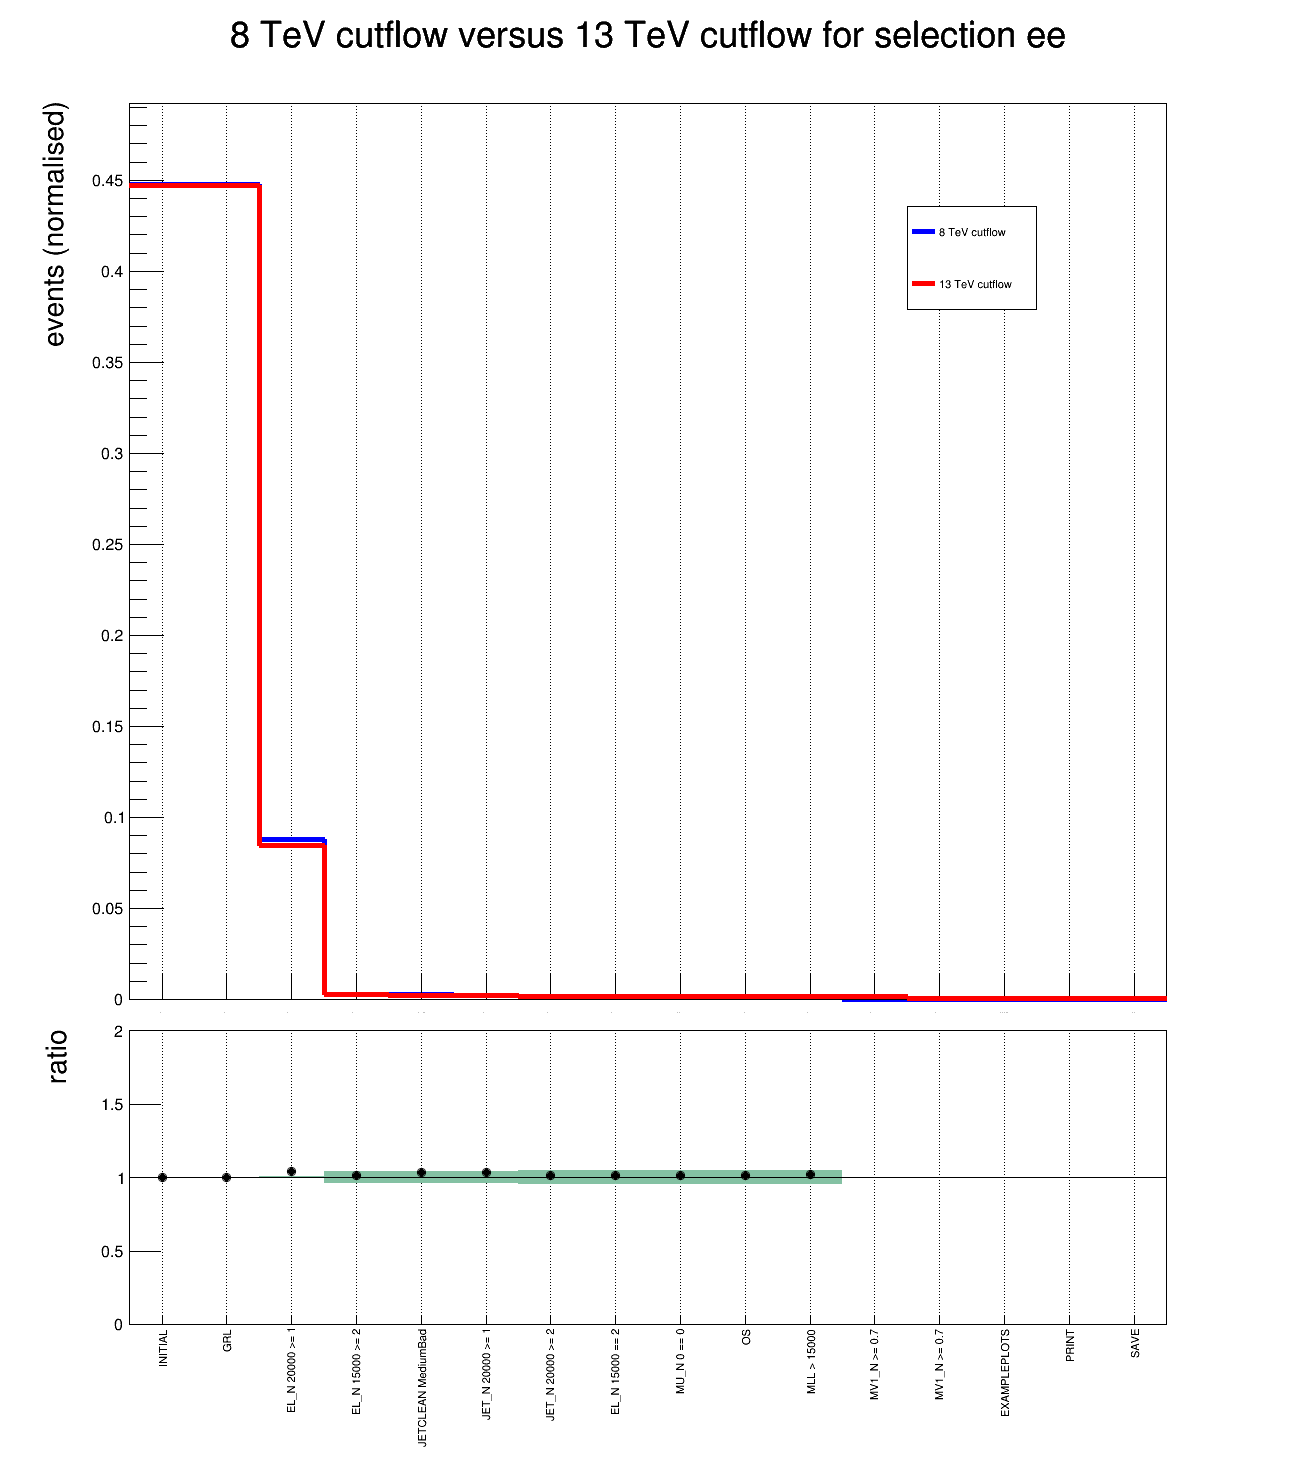
\includegraphics[width=\measureMSpecification]{\directoryImagesB/2015-04-21T0410Z_cutflow_ee.png}&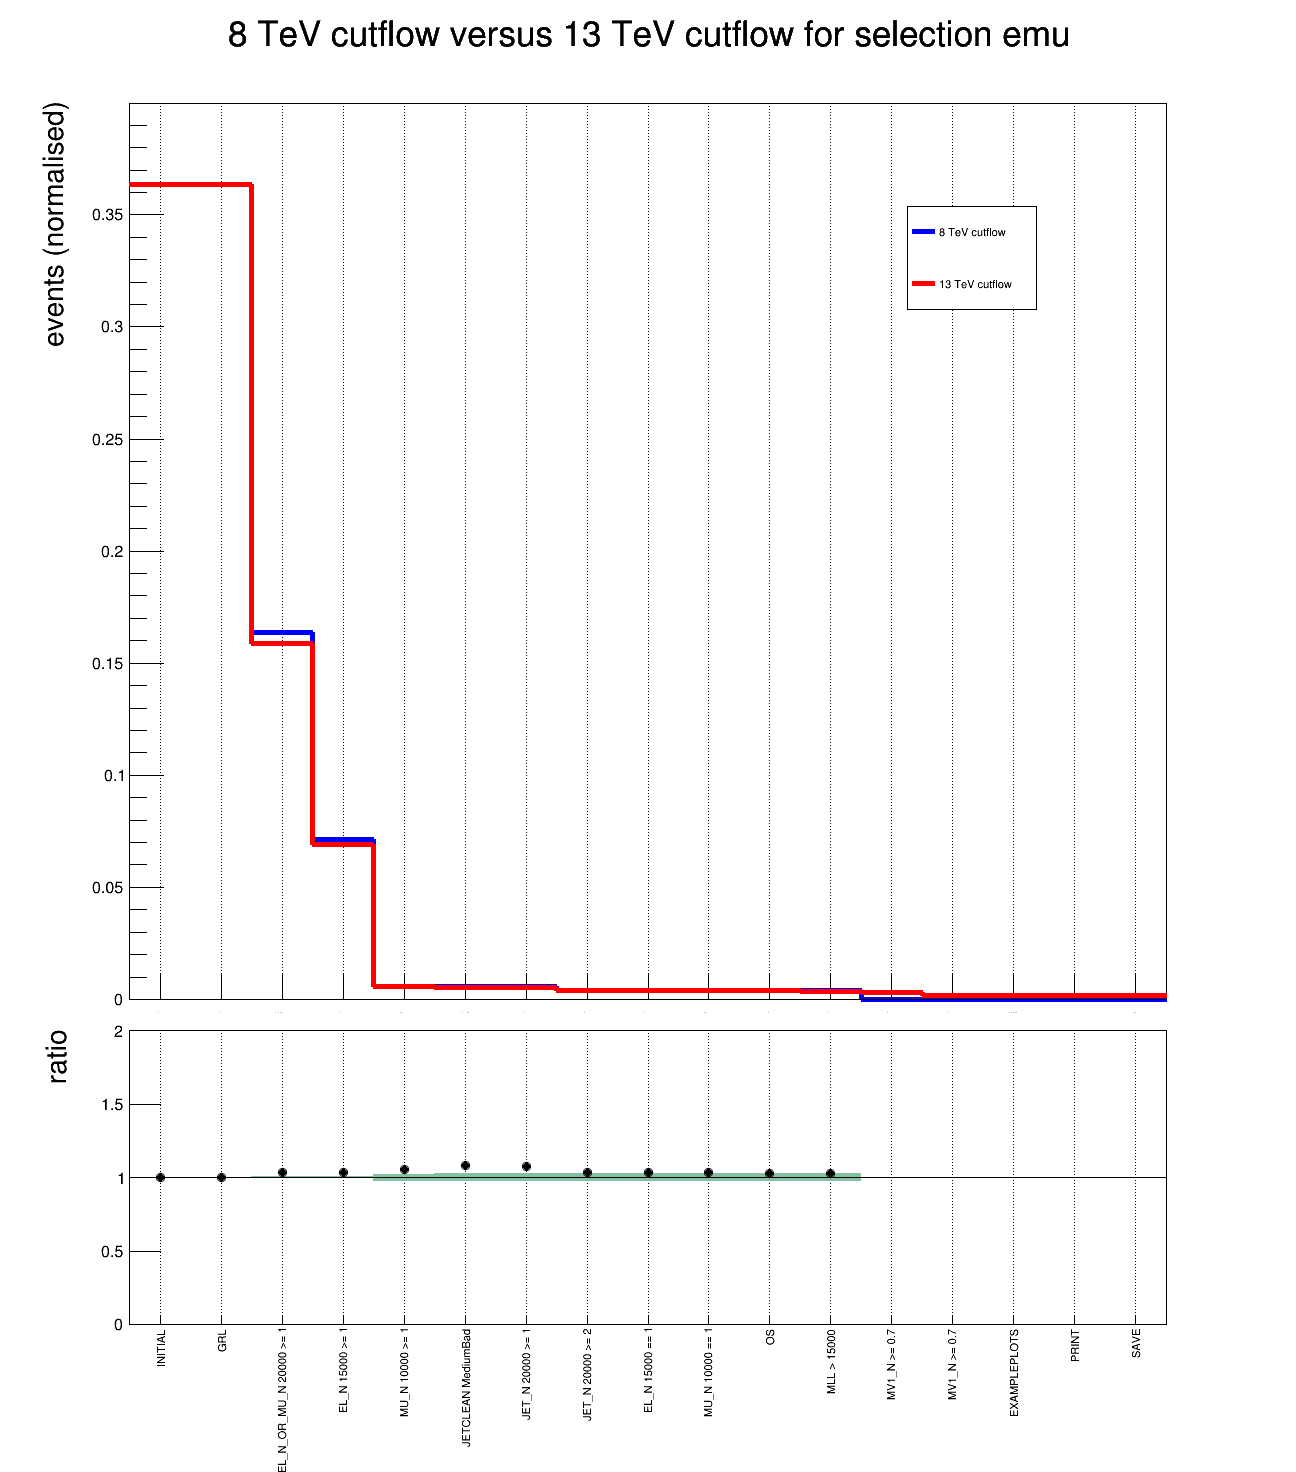
\includegraphics[width=\measureMSpecification]{\directoryImagesB/2015-04-21T0410Z_cutflow_emu.png}&
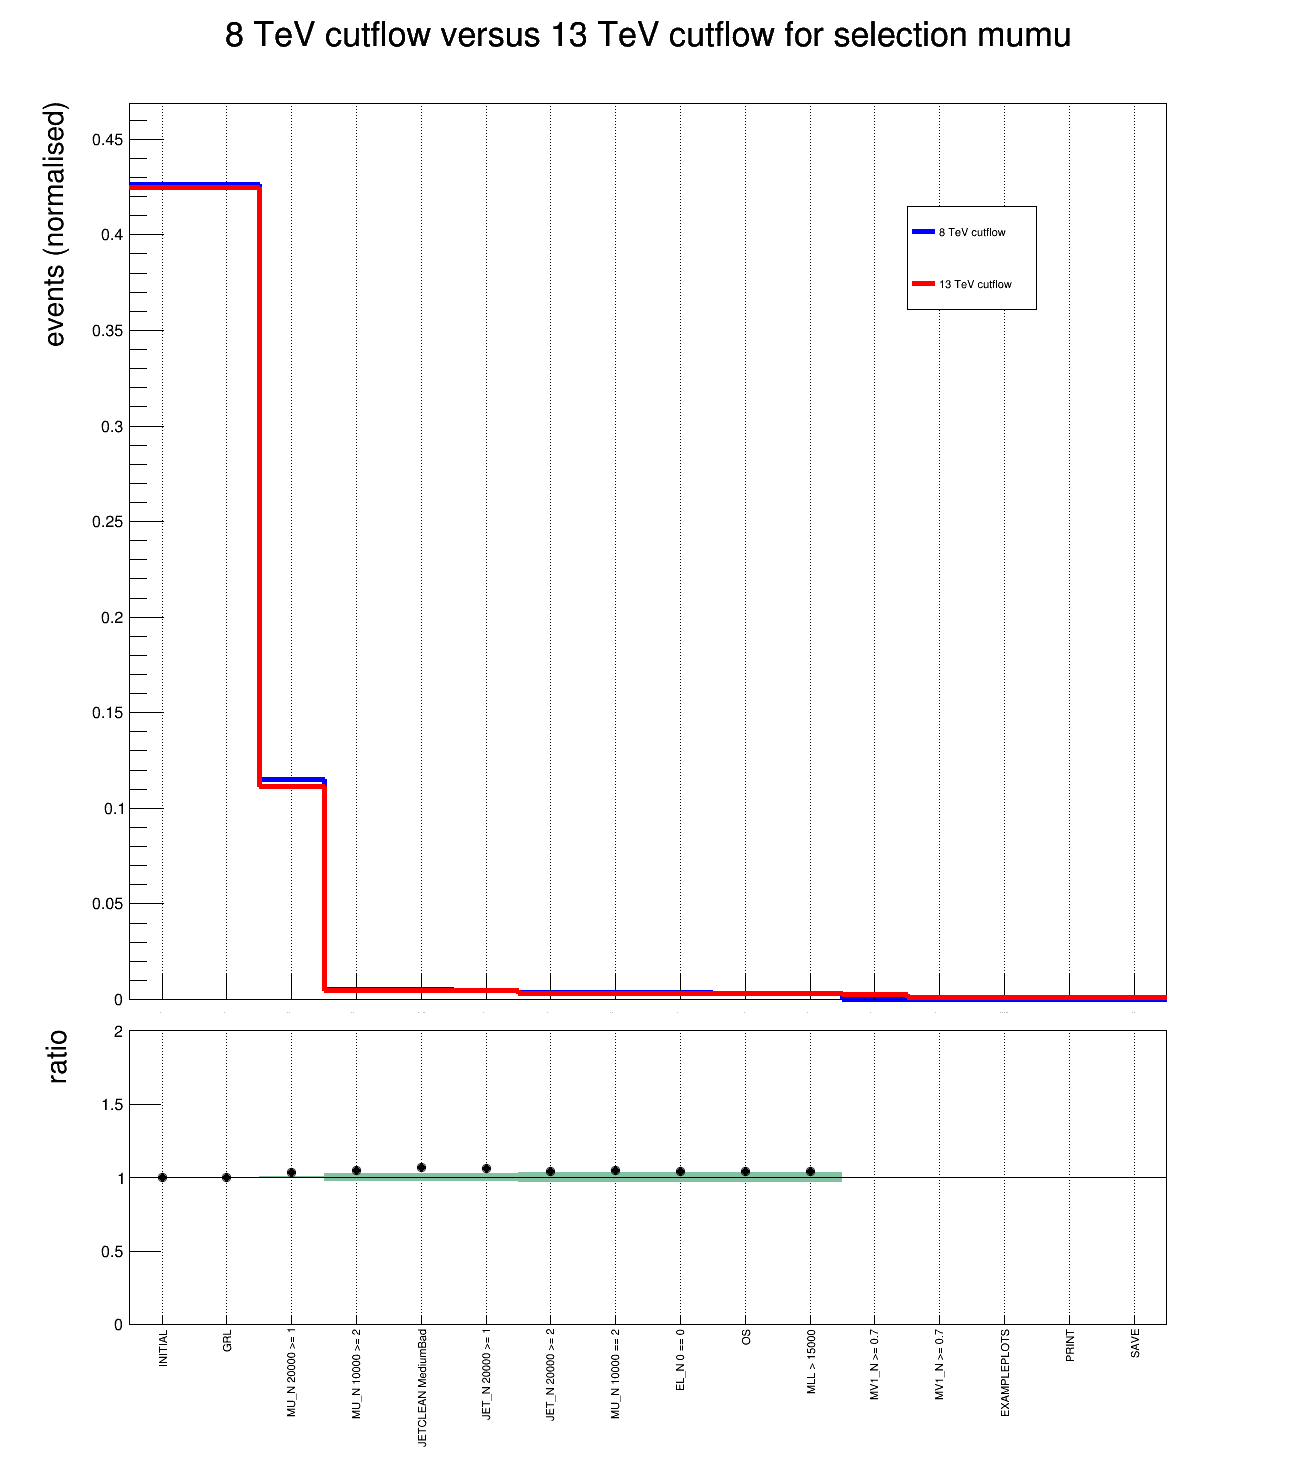
\includegraphics[width=\measureMSpecification]{\directoryImagesB/2015-04-21T0410Z_cutflow_mumu.png}\\
\end{tabular}
\vspace{0.5 cm}\\I3PD+SV1: \url{https://indico.cern.ch/event/387410/contribution/9/material/slides/0.pdf}
\end{center}
\end{frame}

\begin{frame}
\frametitle{${8\textrm{ TeV}}$ vs.~${13\textrm{ TeV}}$: centrality}
\begin{center}
\begin{tabular}{cc}
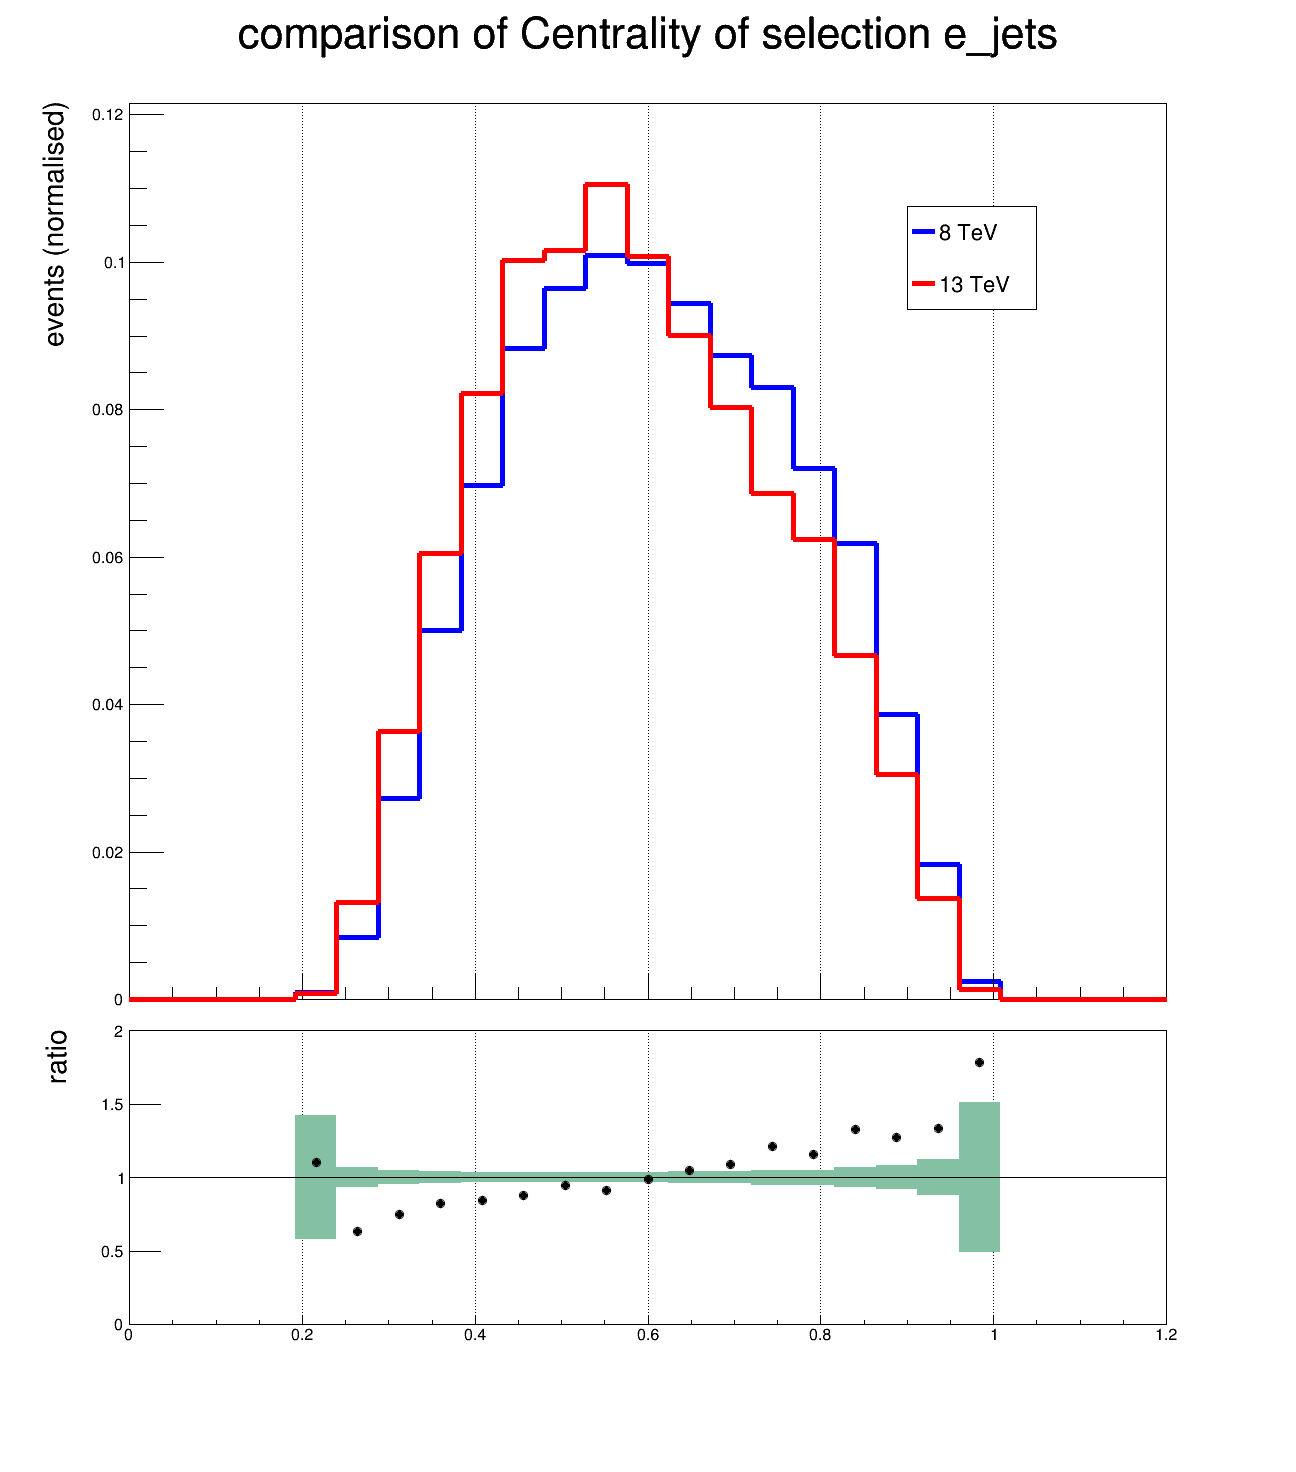
\includegraphics[width=\measureNSpecification]{\directoryImagesB/2015-04-21T0410Z_comparison_of_Centrality_of_selection_e_jets.png}&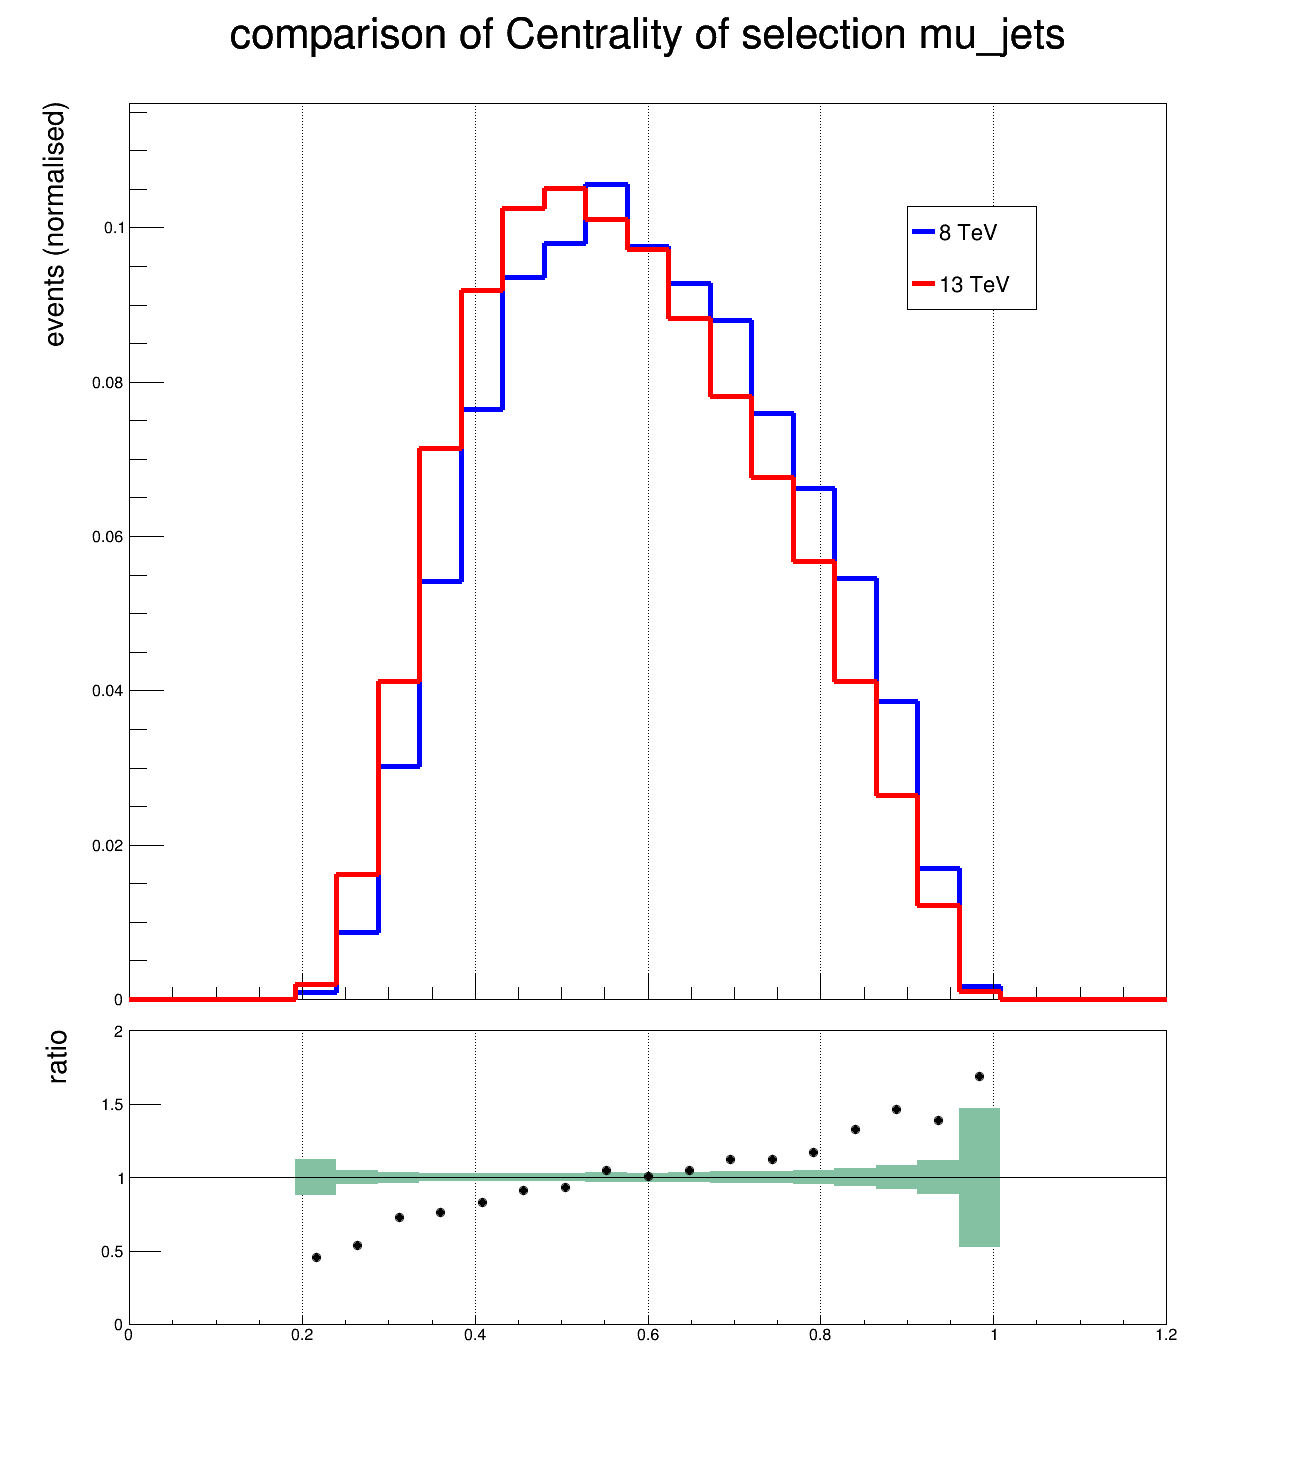
\includegraphics[width=\measureNSpecification]{\directoryImagesB/2015-04-21T0410Z_comparison_of_Centrality_of_selection_mu_jets.png}\\
\end{tabular}
\end{center}
\end{frame}

\begin{frame}
\frametitle{${8\textrm{ TeV}}$ vs.~${13\textrm{ TeV}}$: JVF}
\begin{center}
\begin{tabular}{cc}
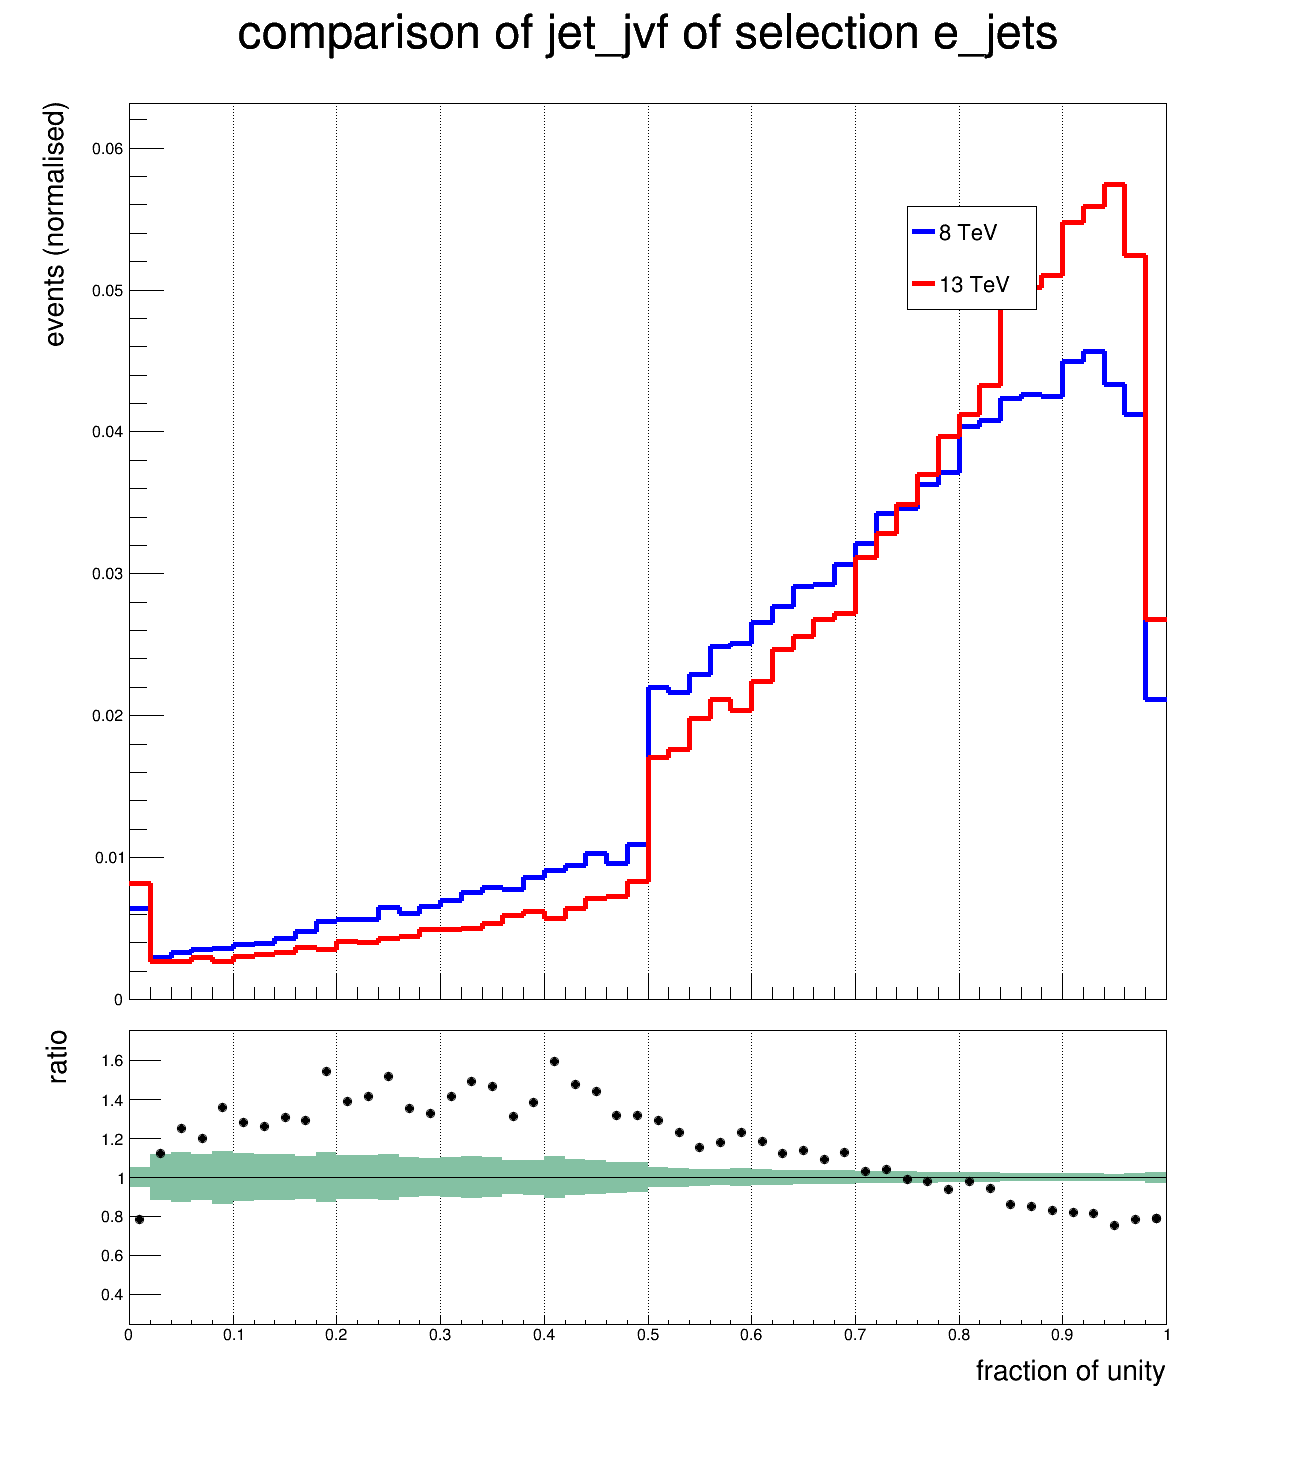
\includegraphics[width=\measureNSpecification]{\directoryImagesB/2015-04-21T0410Z_comparison_of_jet_jvf_of_selection_e_jets.png}&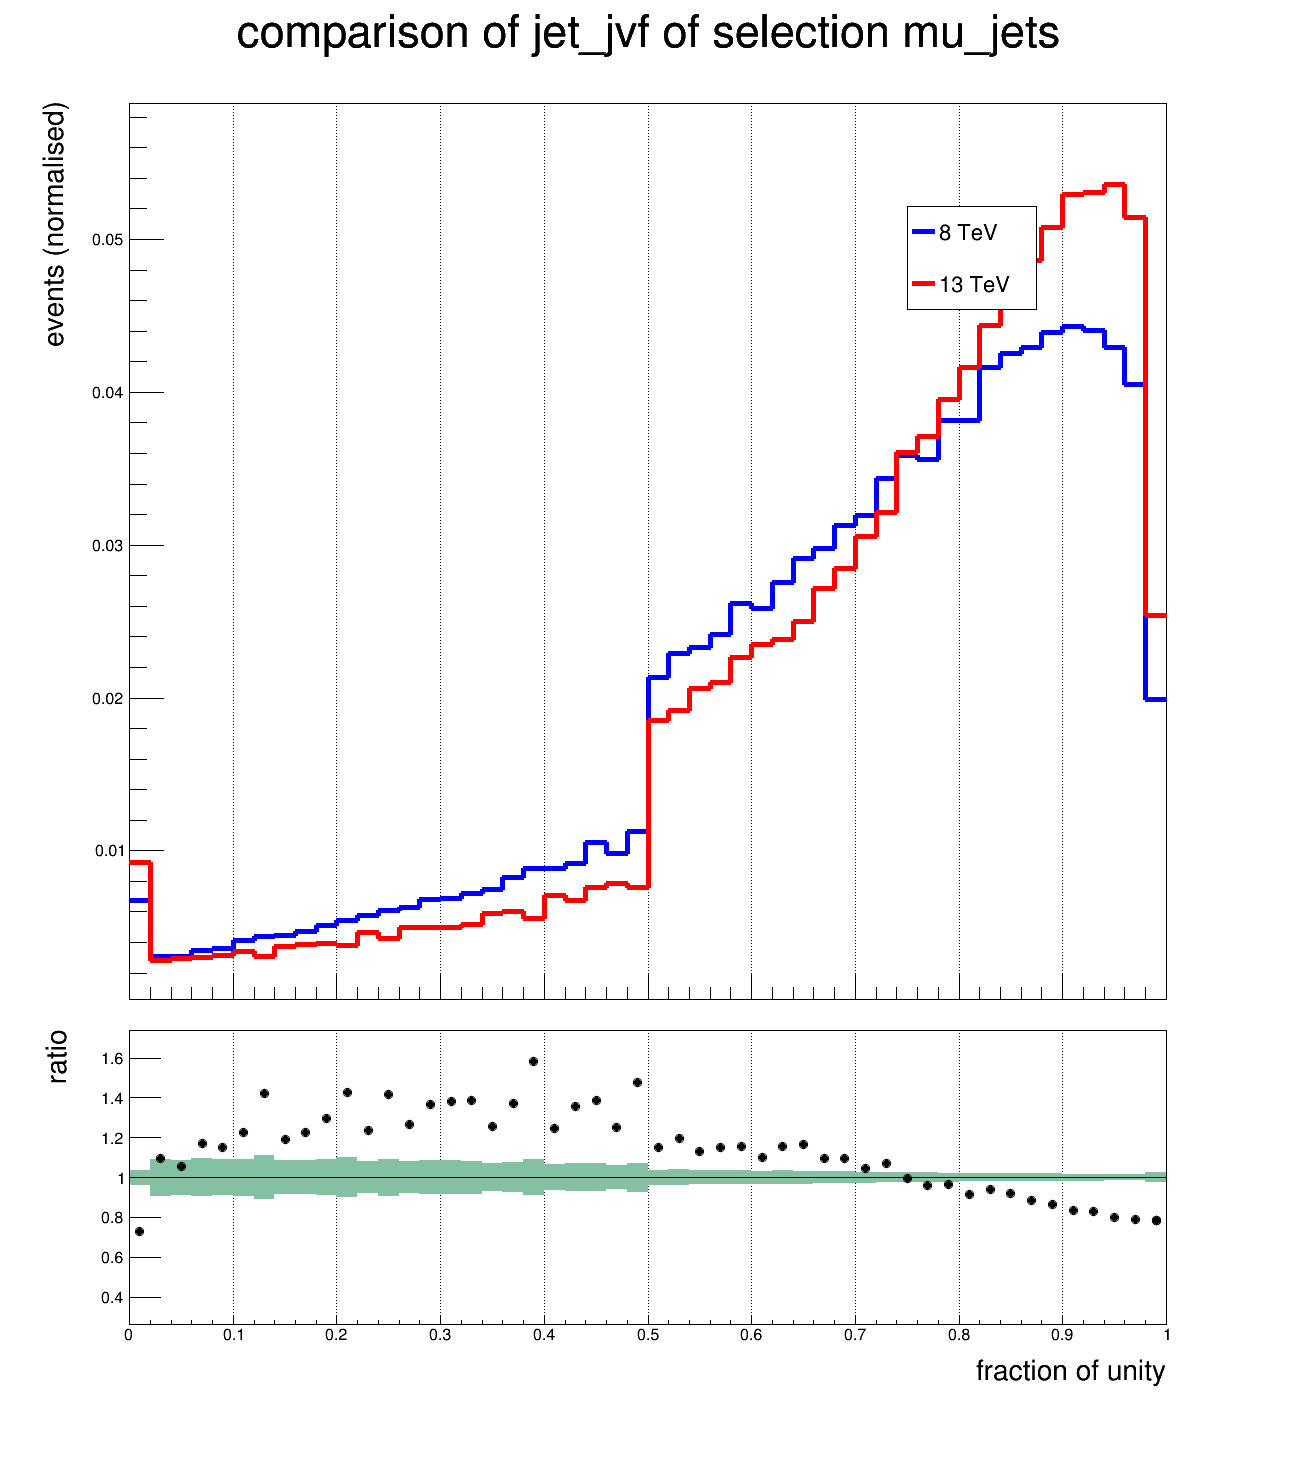
\includegraphics[width=\measureNSpecification]{\directoryImagesB/2015-04-21T0410Z_comparison_of_jet_jvf_of_selection_mu_jets.png}\\
\end{tabular}
\end{center}
\end{frame}

\begin{frame}
\frametitle{${8\textrm{ TeV}}$ vs.~${13\textrm{ TeV}}$: subleading jets ${p_{T}}$ of ${e}$ selection}
\begin{center}
\begin{tabular}{ccc}
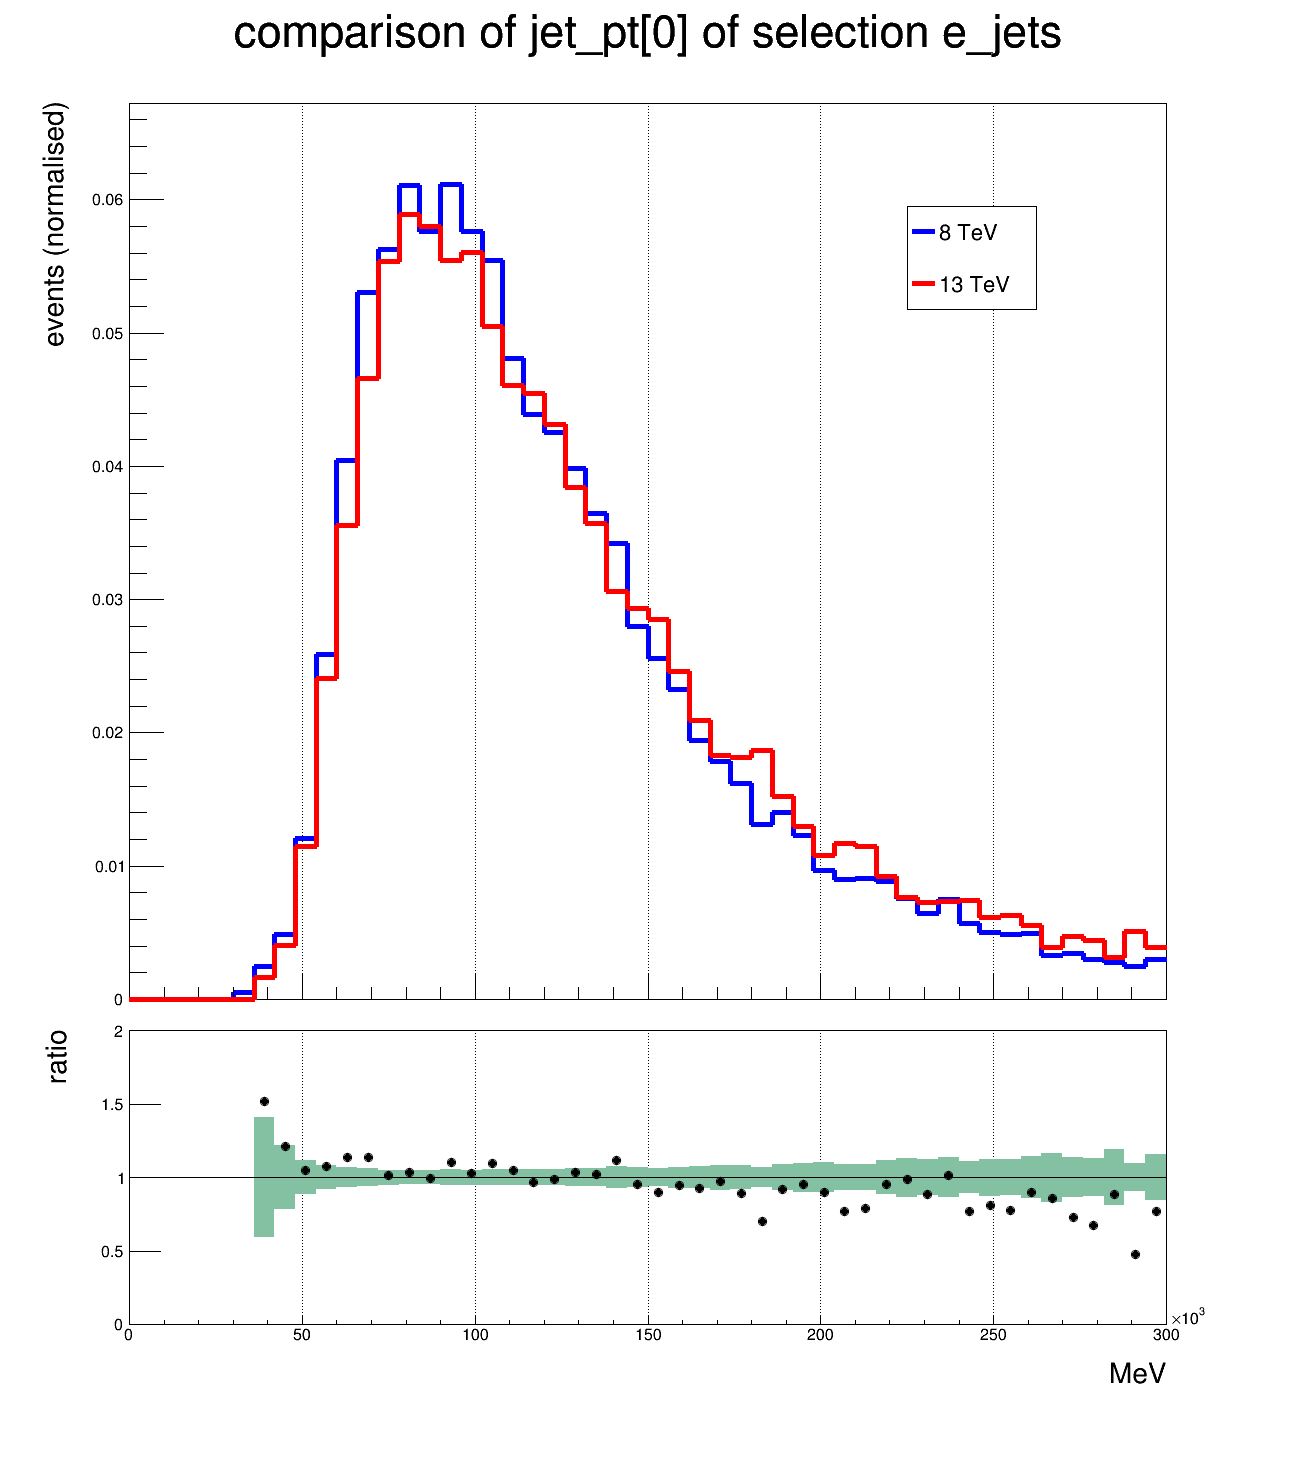
\includegraphics[width=\measureLSpecification]{\directoryImagesB/2015-04-21T0410Z_comparison_of_jet_pt[0]_of_selection_e_jets.png}&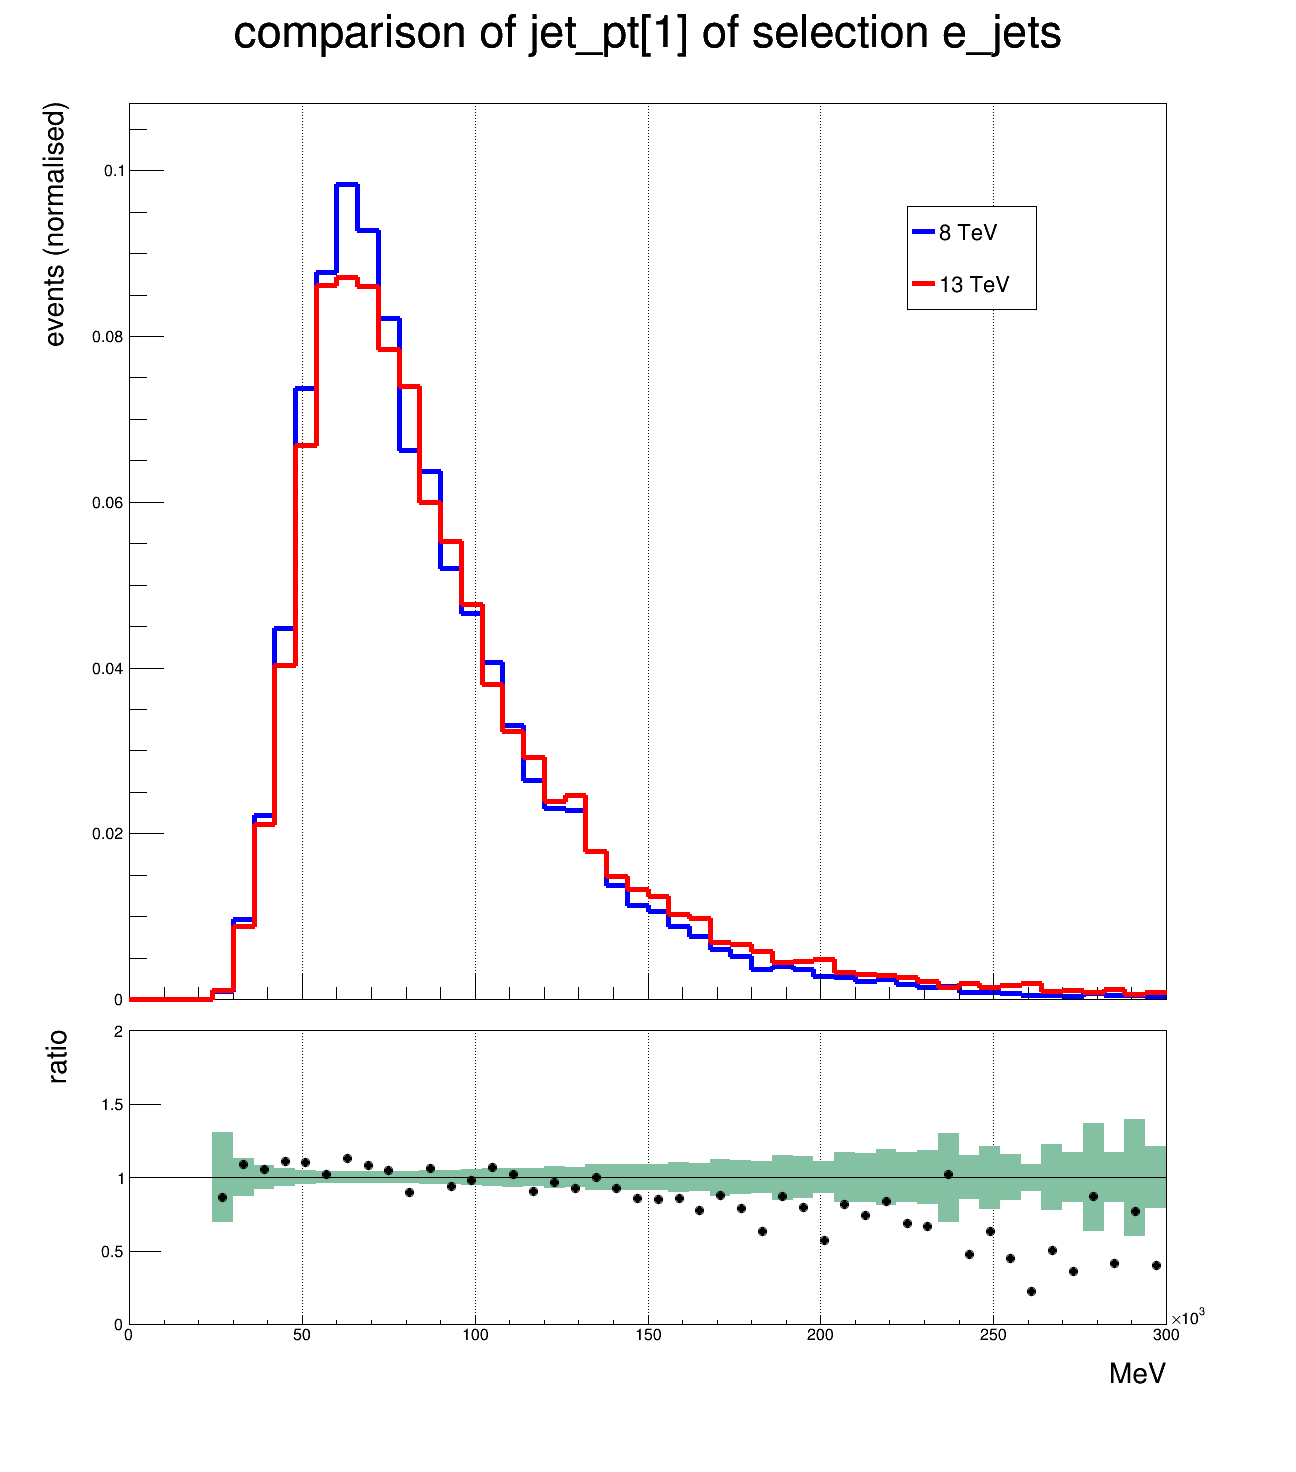
\includegraphics[width=\measureLSpecification]{\directoryImagesB/2015-04-21T0410Z_comparison_of_jet_pt[1]_of_selection_e_jets.png}&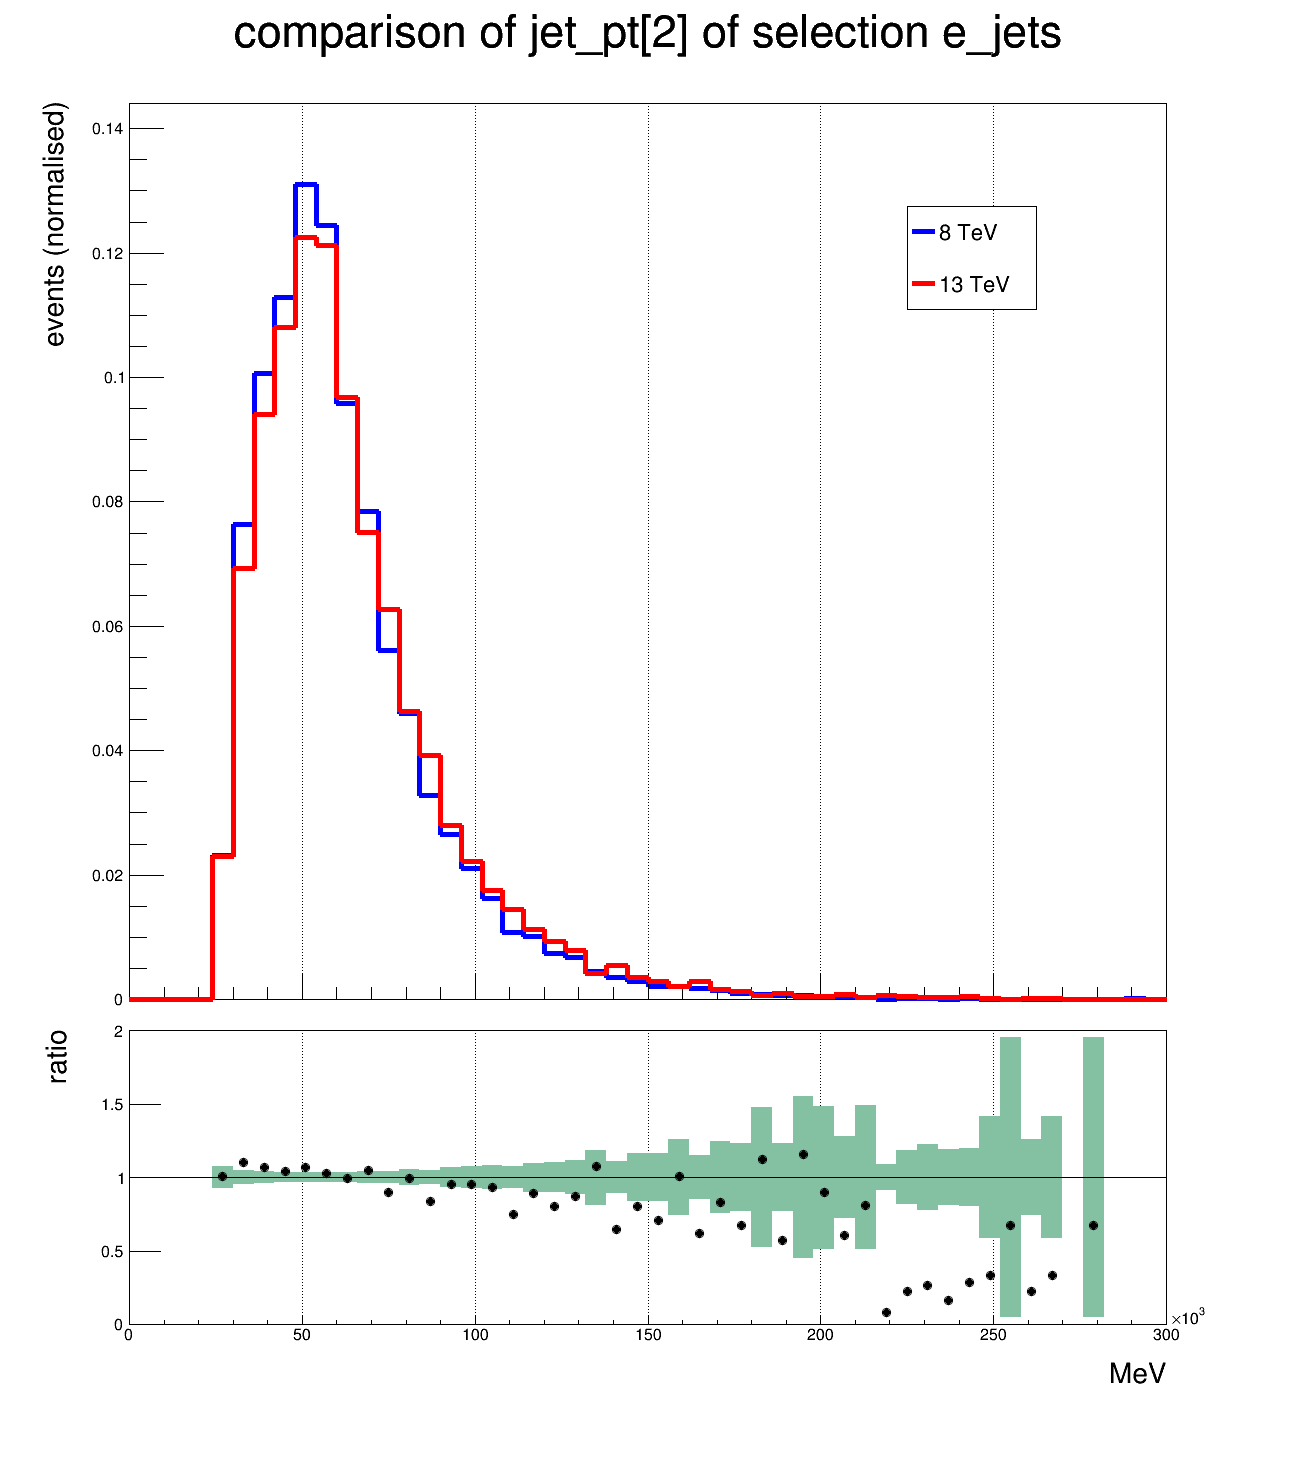
\includegraphics[width=\measureLSpecification]{\directoryImagesB/2015-04-21T0410Z_comparison_of_jet_pt[2]_of_selection_e_jets.png}\\
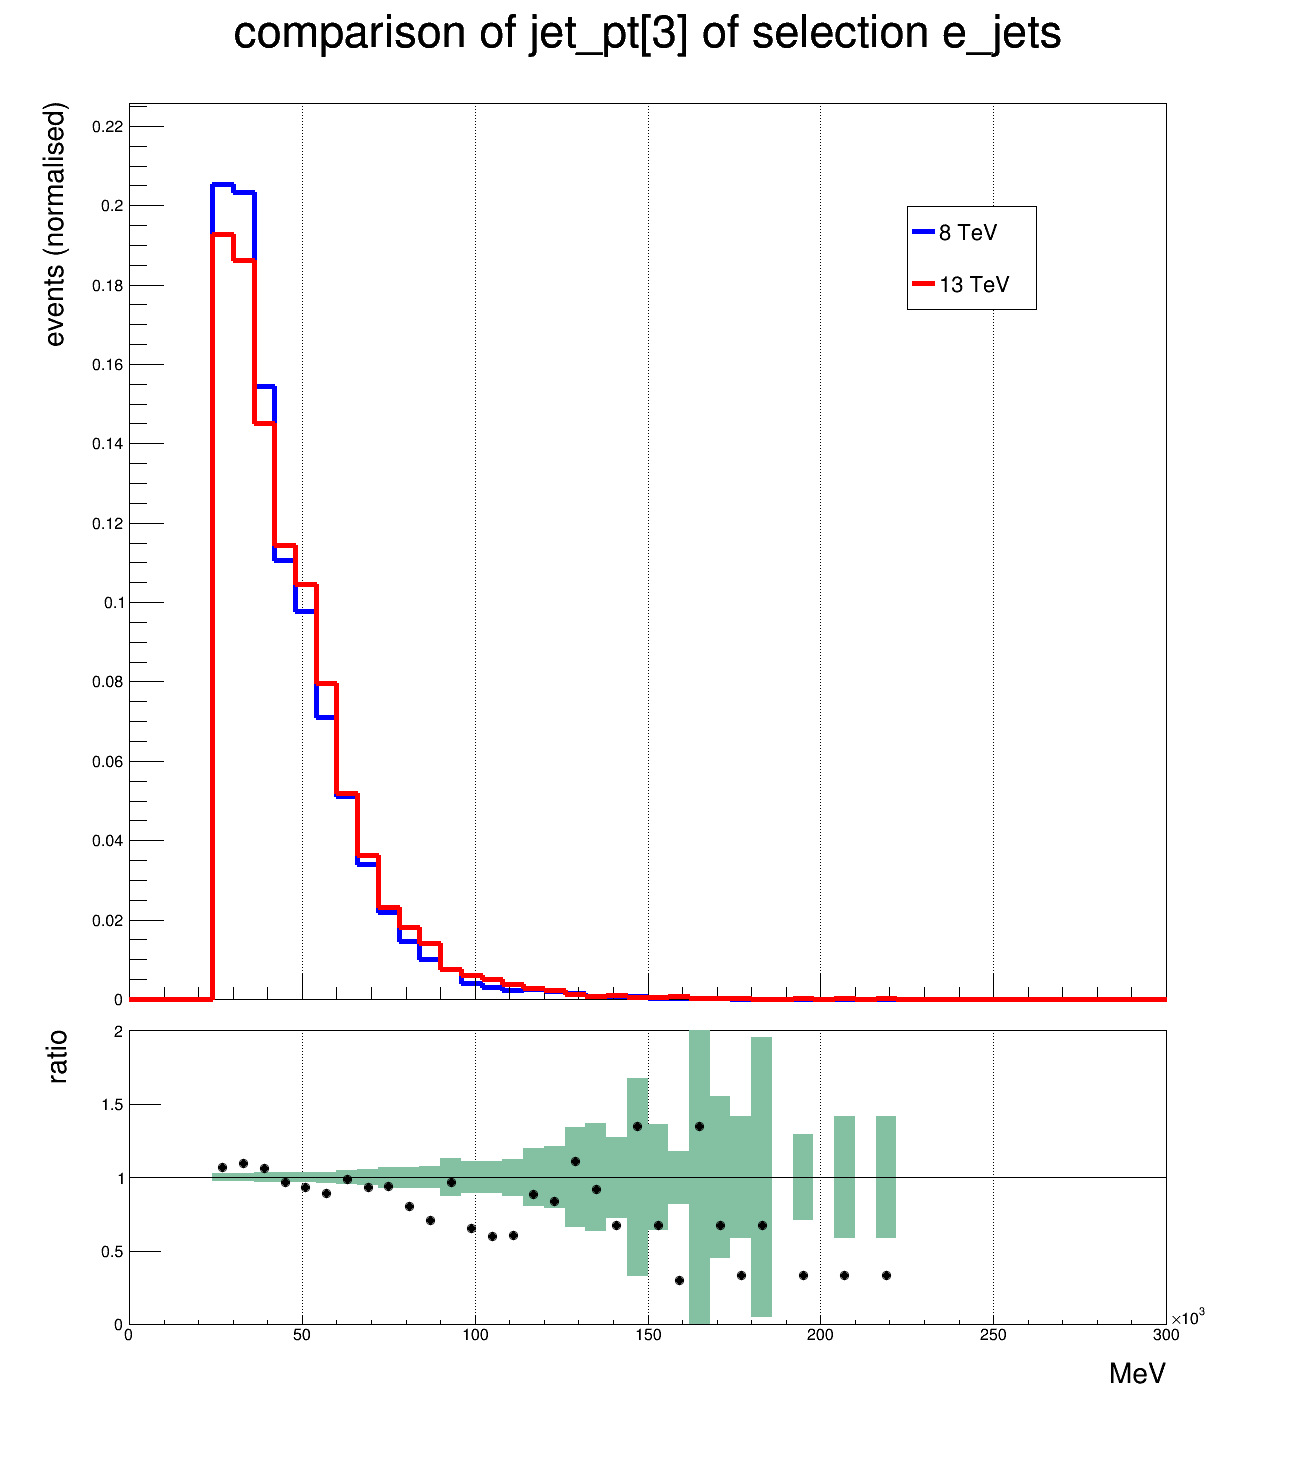
\includegraphics[width=\measureLSpecification]{\directoryImagesB/2015-04-21T0410Z_comparison_of_jet_pt[3]_of_selection_e_jets.png}&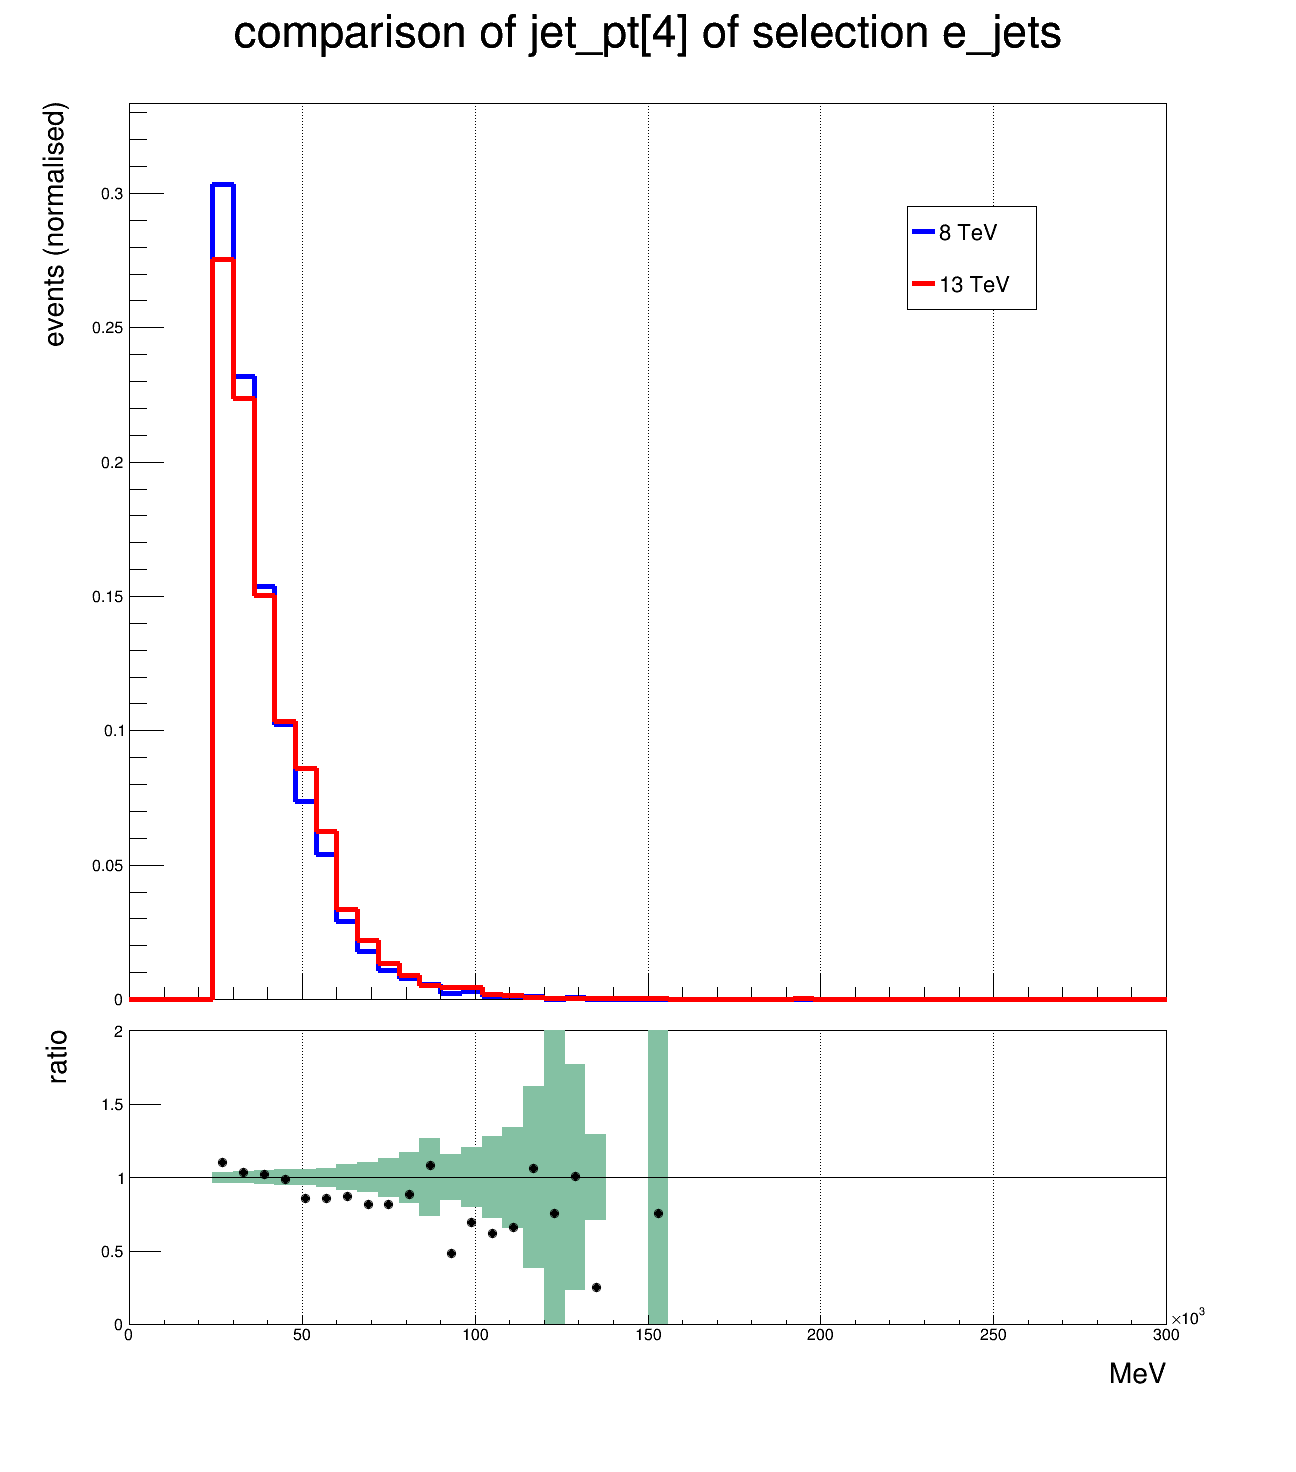
\includegraphics[width=\measureLSpecification]{\directoryImagesB/2015-04-21T0410Z_comparison_of_jet_pt[4]_of_selection_e_jets.png}&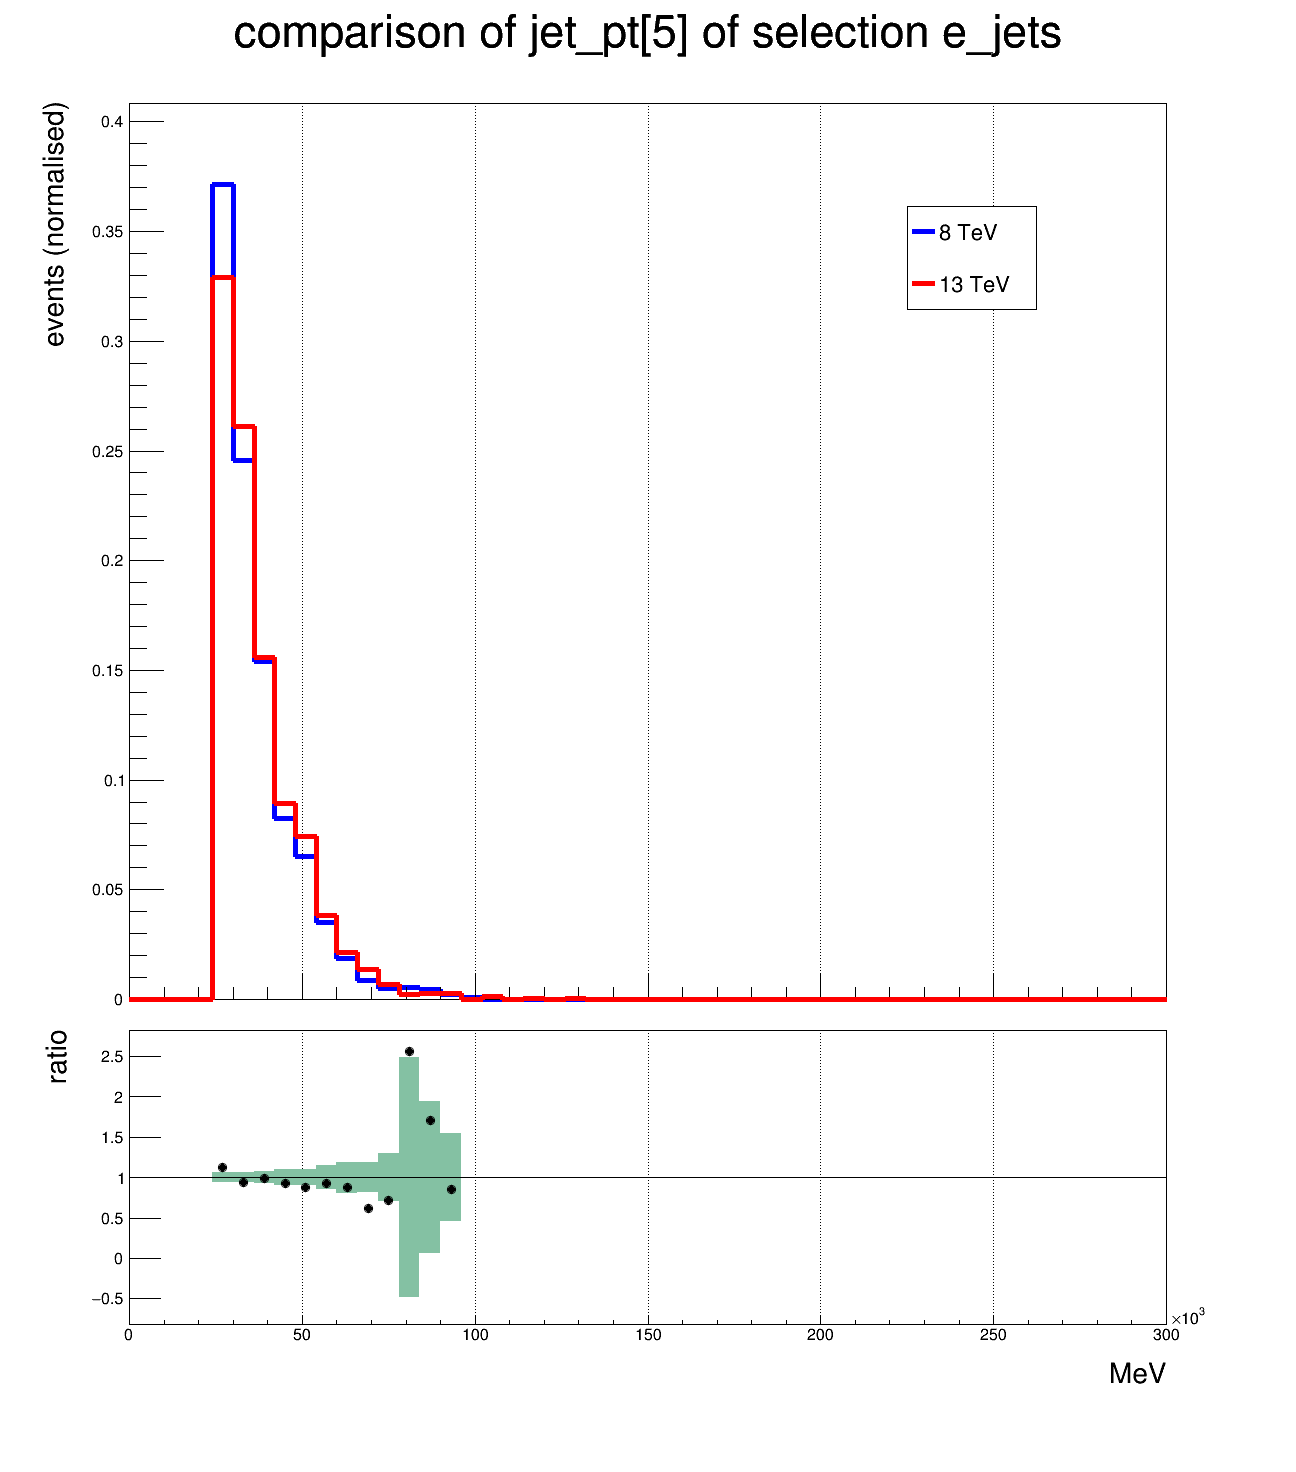
\includegraphics[width=\measureLSpecification]{\directoryImagesB/2015-04-21T0410Z_comparison_of_jet_pt[5]_of_selection_e_jets.png}\\
\end{tabular}
\end{center}
\end{frame}

\begin{frame}{${p_{T}}$ ratio results for training with epochs of interest}
\begin{table}[h]
\begin{tabular}{cc}
40 epochs:&100 epochs:
\\
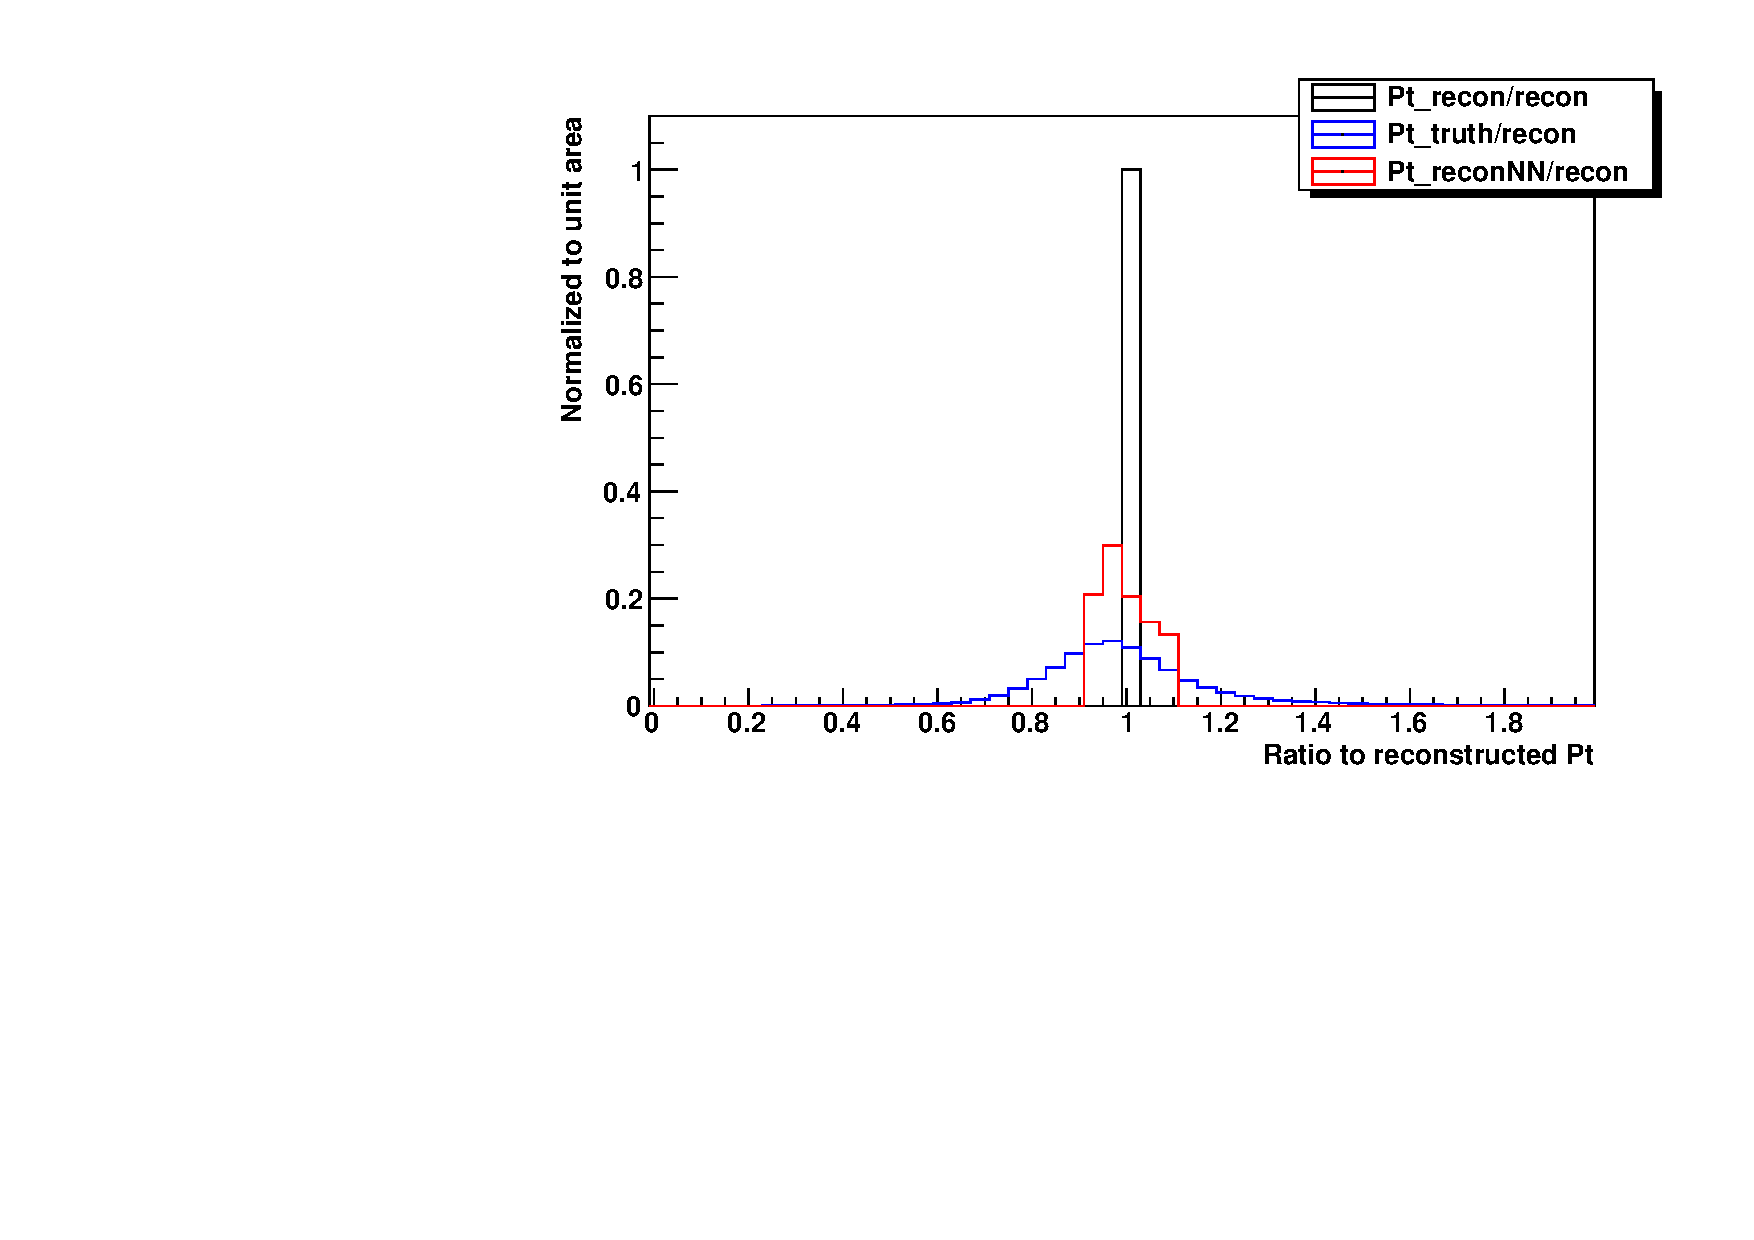
\includegraphics[width=\measureMSpecification]{\directoryImagesB/wMwN_atlas_125_all_NN_rEt_rSumPtTrk_rWidth5trPt_40_plots_corrected_Pt_train_ratio.pdf}
&
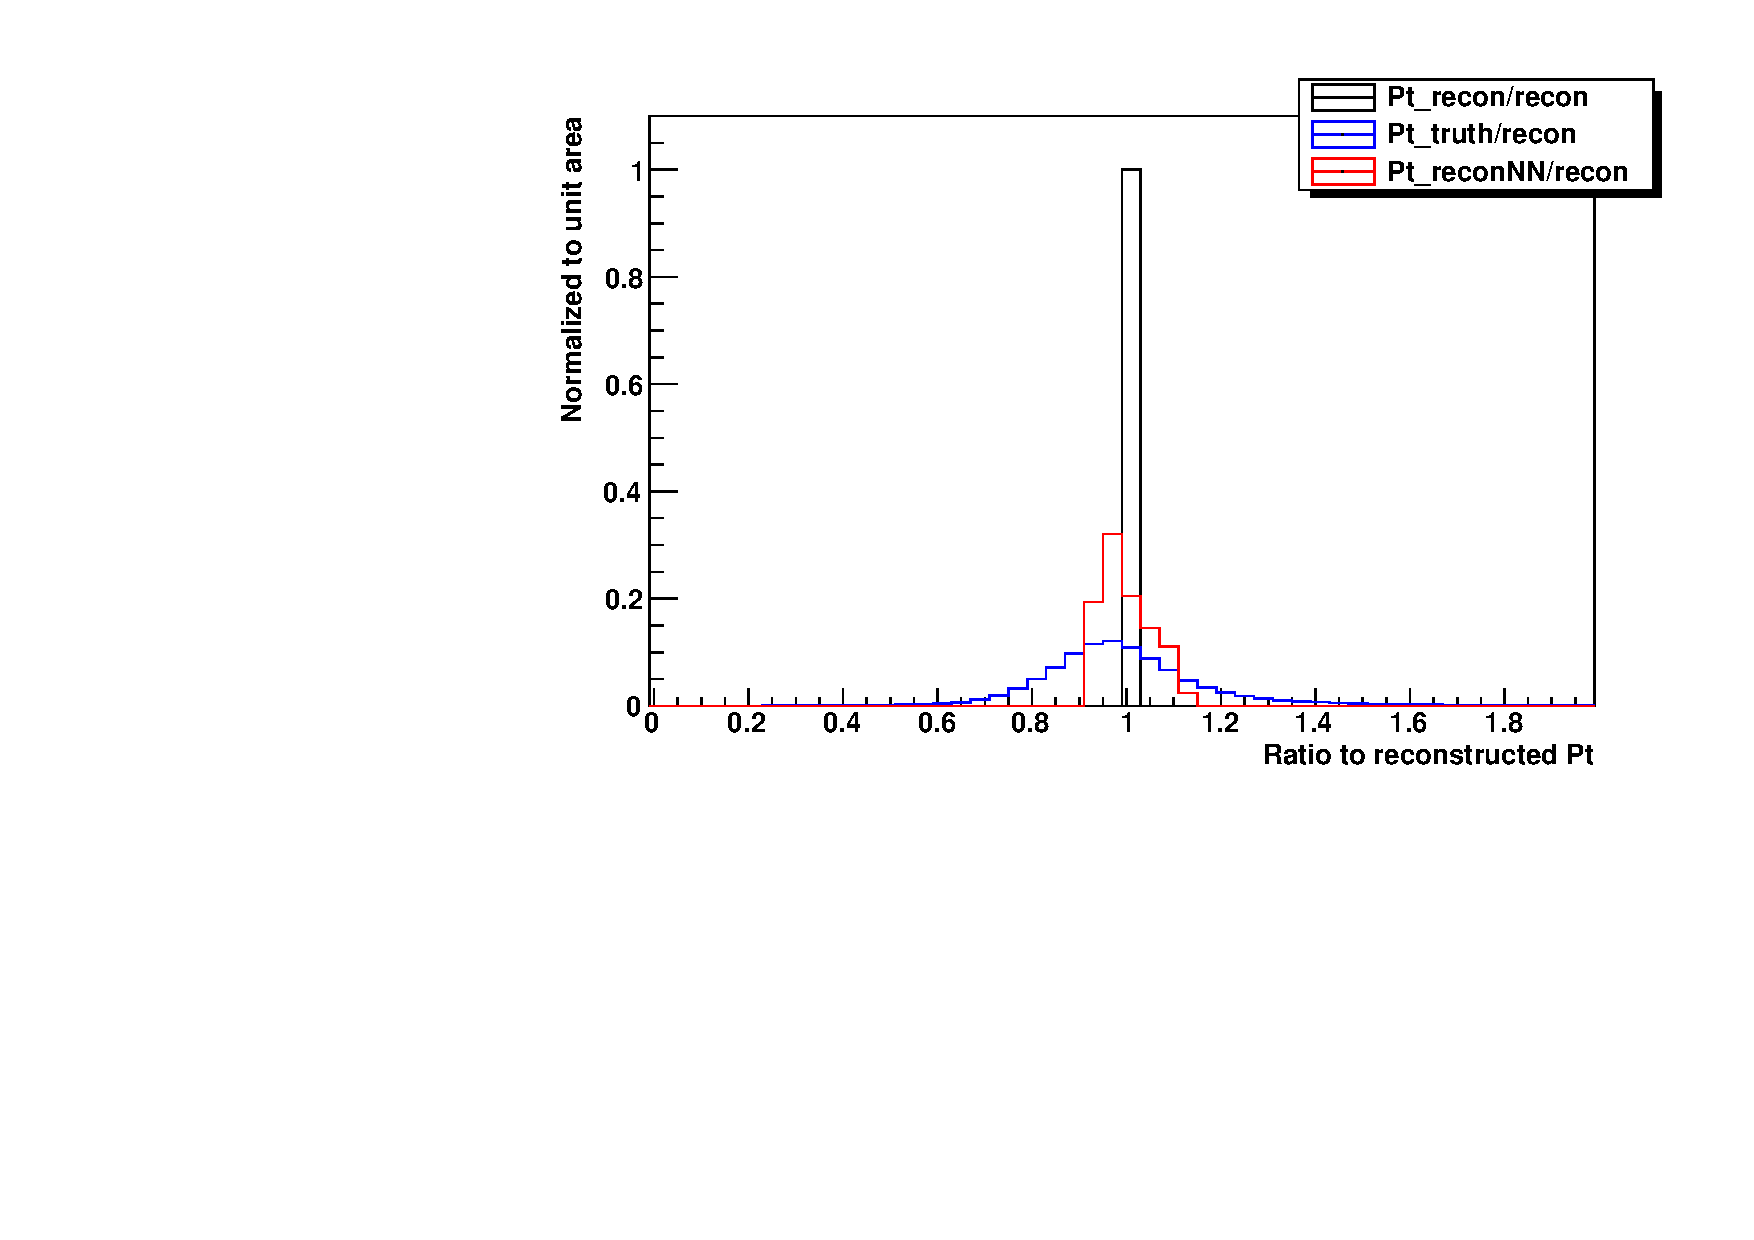
\includegraphics[width=\measureMSpecification]{\directoryImagesB/wMwN_atlas_125_all_NN_rEt_rSumPtTrk_rWidth5trPt_100_plots_corrected_Pt_train_ratio.pdf}
\\
145 epochs:&300 epochs:
\\
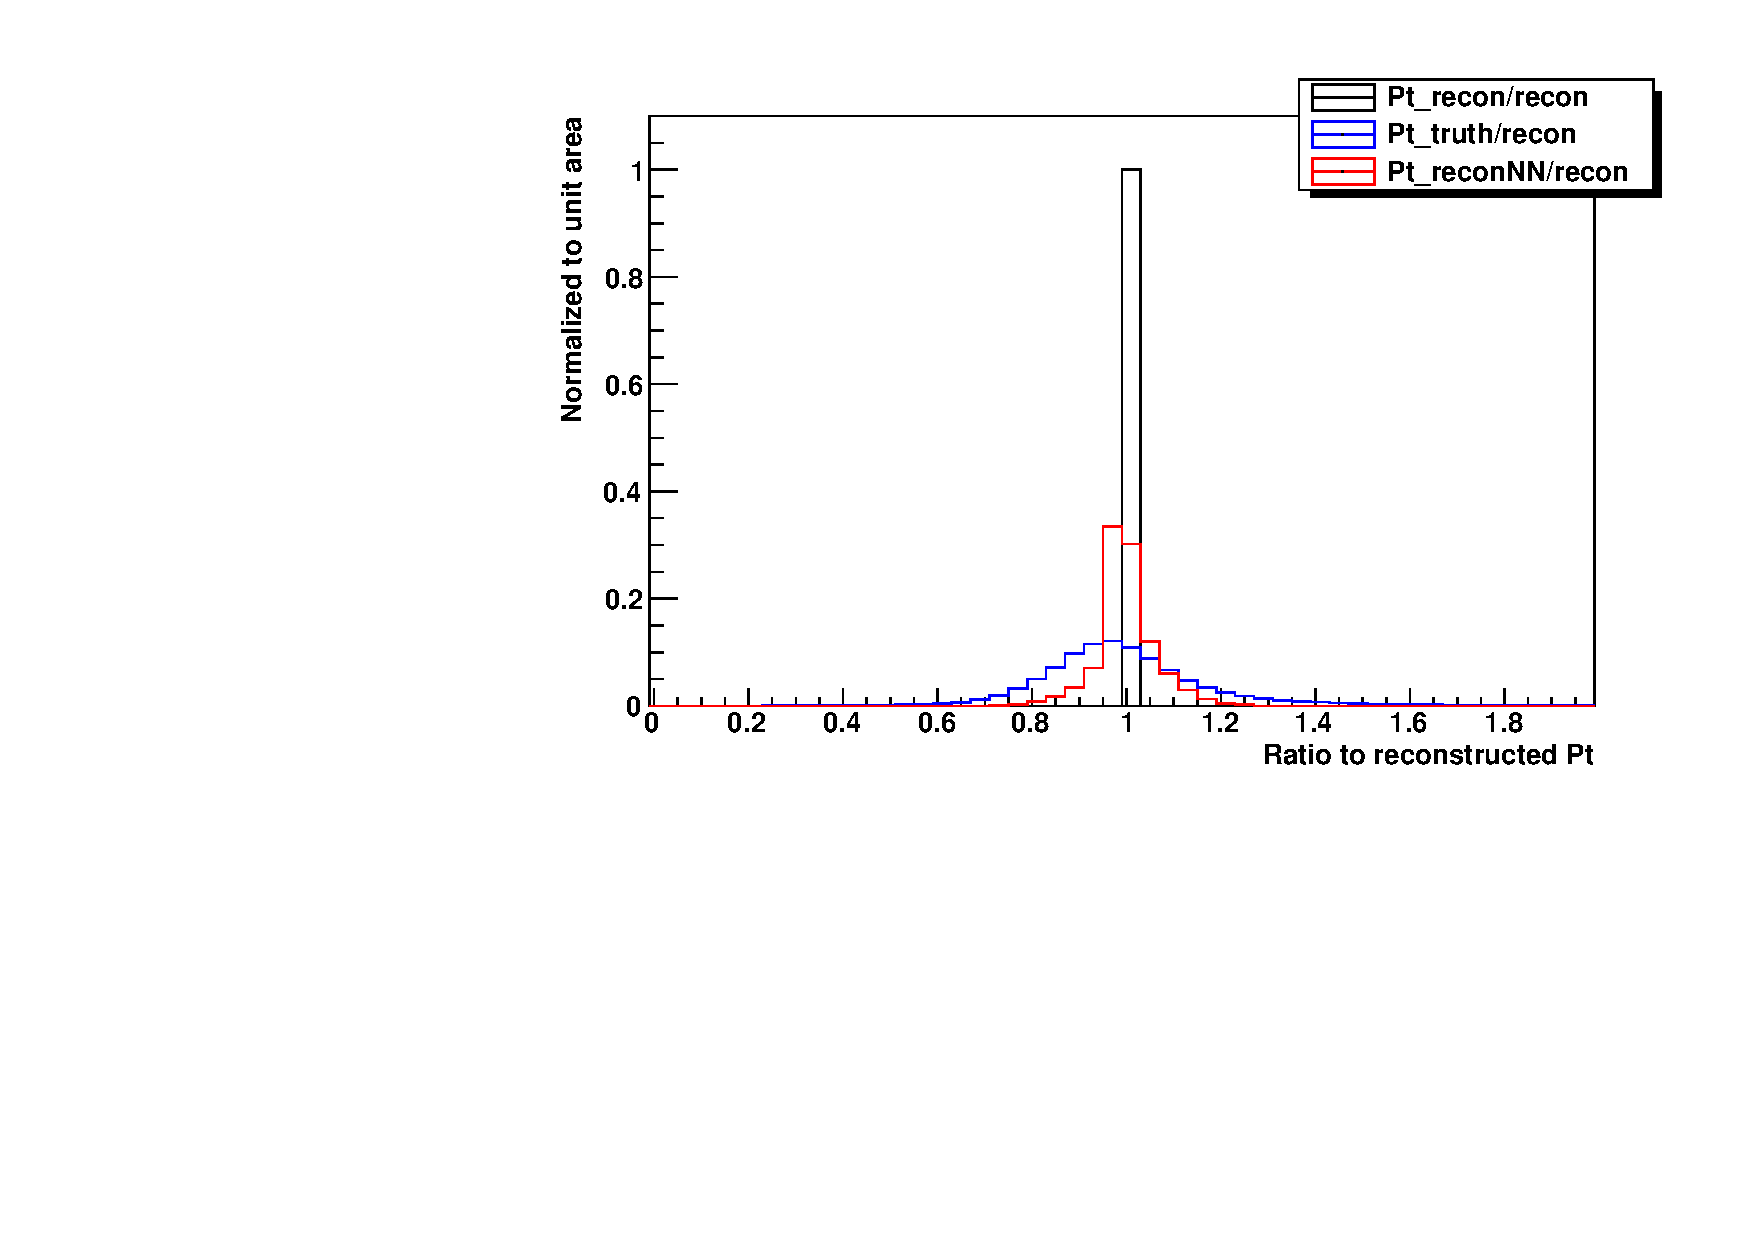
\includegraphics[width=\measureMSpecification]{\directoryImagesB/wMwN_atlas_125_all_NN_rEt_rSumPtTrk_rWidth5trPt_145_plots_corrected_Pt_train_ratio.pdf}
&
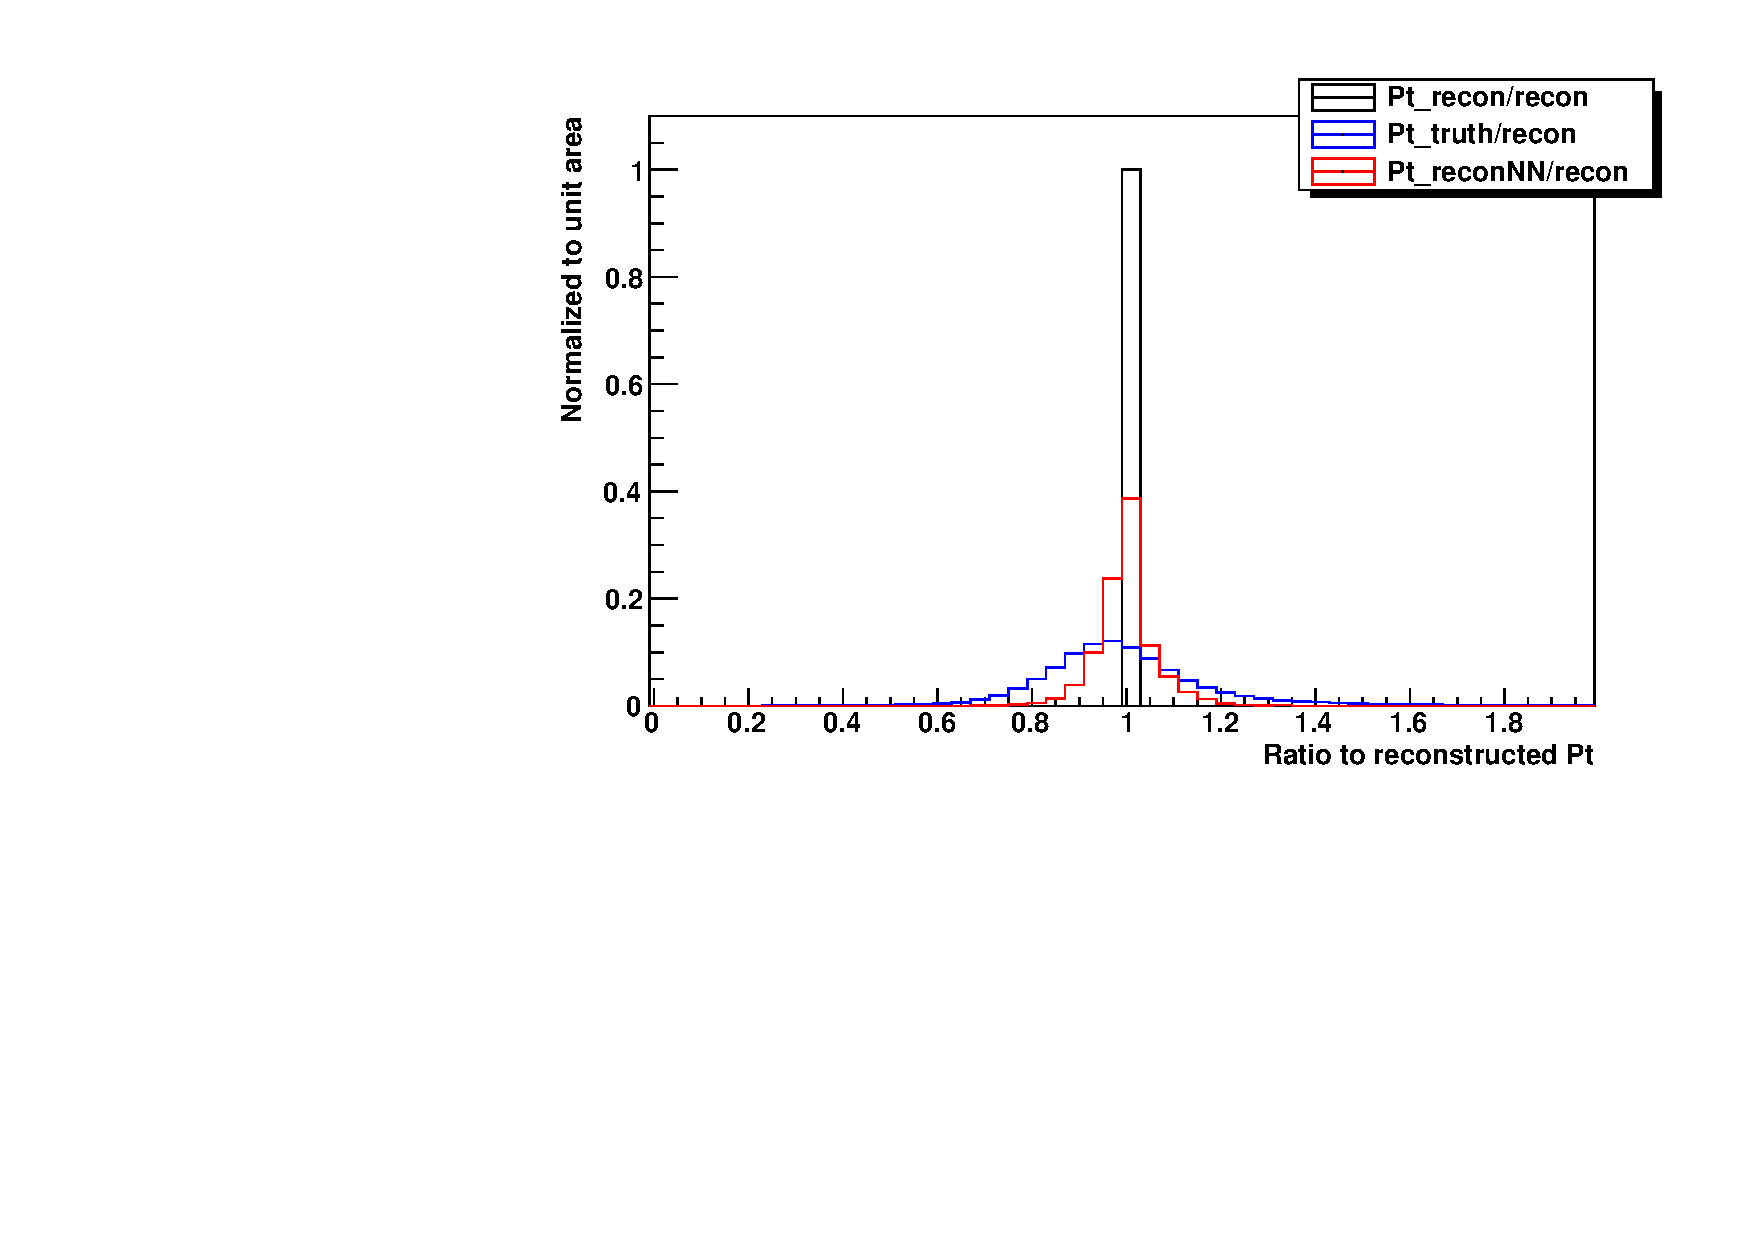
\includegraphics[width=\measureMSpecification]{\directoryImagesB/wMwN_atlas_125_all_NN_rEt_rSumPtTrk_rWidth5trPt_300_plots_corrected_Pt_train_ratio.pdf}
\\
\end{tabular}
\end{table}
\end{frame}

\begin{frame}{neural networks and input variables}
Four neural networks with progressively increasing input information were defined, all trained through 250 epochs (training cycles). NN0 comprises only the ${\mu}$-in-jet and ${p_{T}}$-only NN corrections, as opposed to further NN corrections.
\begin{center}
\resizebox{11.5 cm}{!}{
\begin{tabular}{ll}
\hline\hline
neural network designation&input variables\\
\hline
NN0&no new neural network applied\\
NN1&Et, SumPtTrk, Width\\
NN2&Et, SumPtTrk, Width, MET\\
NN3&Et, SumPtTrk, Width, MET, METPhi, JetPhi\\
\hline\hline
\end{tabular}
}
\end{center}
\end{frame}

\begin{frame}
\frametitle{per-event $M_{b\bar{b}}$ resolutions with use of MET direction}
${M_{b\bar{b}}}$ resolutions for ${VH_{b\bar{b}}}$ for progressively decreasing MET energy cut requirements for various neural networks, shown to 3 significant figures:
\begin{center}
\resizebox{11.5 cm}{!}{
\begin{tabular}{llllll}
\hline\hline
selection											&	events	&	NN0		& 	NN1		 & 	NN2 		& NN3\\
\hline
${VH_{b\bar{b}}}$									&	23686	&	0.133	&	0.129	&	0.131	&	0.131\\
${VH_{b\bar{b}}+\textrm{MET}<100\textrm{ GeV}}$		&	22654	&	0.132	&	0.130	&	0.129	&	0.131\\
${VH_{b\bar{b}}+\textrm{MET}<70\textrm{ GeV}}$		&	21094	&	0.131	&	0.128	&	0.129	&	0.129\\
${VH_{b\bar{b}}+\textrm{MET}<40\textrm{ GeV}}$		&	15050	&	0.128	&	0.126	&	0.126	&	0.126\\
${VH_{b\bar{b}}+\textrm{MET}<20\textrm{ GeV}}$		&	6174	&	0.130	&	0.127	&	0.126	&	0.127\\
\hline\hline
\end{tabular}
}
\end{center}
\end{frame}

\begin{frame}
\frametitle{per event ${M_{b\bar{b}}}$ resolutions with use of MET direction}
\small Here, the physical processes are ranked according to the effectiveness of the corresponding behaviour they induce in NN3, where a greater effectiveness is taken to mean a smaller resolution value. \emph{Caveat:} Systematic uncertainties are not given their due consideration.
\begin{center}
\resizebox{11.5 cm}{!}{
\begin{tabular}{llllll}
\hline\hline
selection															&	events	&	NN0			& 	NN1			 & 	NN2 		& NN3\\
\hline
\textcolor{red}{${VH_{b\bar{b}}+\textrm{MET}>100\textrm{ GeV}}$}	&	1032	&	0.121542	&	0.129038	&	0.13072		&	\textcolor{red}{0.116975}\\
\textcolor{red}{${VH_{b\bar{b}}+\textrm{MET}<40\textrm{ GeV}}$}		&	15050	&	0.128387	&	0.125939	&	0.125637	&	\textcolor{red}{0.125963}\\				
\textcolor{red}{${VH_{b\bar{b}}+\textrm{MET}<20\textrm{ GeV}}$}		&	6174	&	0.129539	&	0.127454	&	0.126029	&	\textcolor{red}{0.127043}\\
\textcolor{red}{${VH_{b\bar{b}}+\textrm{MET}<70\textrm{ GeV}}$}		&	21094	&	0.131248	&	0.128119	&	0.128908	&	\textcolor{red}{0.128825}\\
\textcolor{red}{${VH_{b\bar{b}}+\textrm{MET}<100\textrm{ GeV}}$}	&	22654	&	0.132004	&	0.129924	&	0.129095	&	\textcolor{red}{0.130467}\\
\textcolor{red}{${VH_{b\bar{b}}}$}									&	23686	&	0.132823	&	0.129032	&	0.131202	&	\textcolor{red}{0.131303}\\
\textcolor{red}{${VH_{b\bar{b}}+\textrm{MET}>20\textrm{ GeV}}$}		&	17512	&	0.135974	&	0.13137		&	0.13366		&	\textcolor{red}{0.132341}\\
\textcolor{red}{${VH_{b\bar{b}}+\textrm{MET}>40\textrm{ GeV}}$}		&	8636	&	0.140116	&	0.135415	&	0.140013	&	\textcolor{red}{0.140551}\\
\textcolor{red}{${VH_{b\bar{b}}+\textrm{MET}>70\textrm{ GeV}}$}		&	2592	&	0.143505	&	0.15228		&	0.151469	&	\textcolor{red}{0.155914}\\
\hline\hline
\end{tabular}
}
\end{center}
\end{frame}

\begin{frame}{${m_{b\bar{b}}}$ value results for training with epochs of interest}
${m_{b\bar{b}}}$ resolution results (Gaussian fit) for training with epochs of interest:
\begin{table}[h]
\begin{tabular}{ll|llll|}
\cline{3-6}
&&\multicolumn{4}{c|}{epochs}\\
\cline{3-6}
&&40&100&145&300\\
\hline
\multicolumn{1}{|l|}{\multirow{2}{*}{subset}}	&training&0.137& 0.138&0.138&0.138\\
\multicolumn{1}{|l|}{}							&training test&0.139&0.139&0.139&0.139\\
\hline
\end{tabular}
\end{table}
\end{frame}

\begin{frame}
\frametitle{${m_{b\bar{b}}}$ resolutions with and without MET}
comparison of ${m_{b\bar{b}}}$ resolutions for various channels both excluding and including the MET variable with various epochs:
\begin{table}[ht]
\centering
\resizebox{9.5 cm}{!}{
\begin{tabular}{|l|l|llll|}
\cline{1-1}\cline{3-6}
number of epochs									&				&	${l\nu bb}$	&	${llbb}$	&	${\nu\nu bb}$	&	all\\
\hline
\multicolumn{1}{|c|}{\multirow{3}{*}{50}}			&	without MET	&	0.135159	&	0.138616	&	0.135159		&	0.137488\\
\multicolumn{1}{|c|}{}								&	with MET	&	0.130047	&	0.137266	&	0.136842		&	0.138516\\
						\cline{2-6}
\multicolumn{1}{|c|}{}								&	change		&	-3.78\%		&	-0.97\%		&	+1.24\%			&	+0.75\%\\
\hline
\multicolumn{1}{|c|}{\multirow{3}{*}{100}}			&	without MET	&	0.134537	&	0.138781	&	0.13656			&	0.13743\\
\multicolumn{1}{|c|}{}								&	with MET	&	0.129719	&	0.137265	&	0.136247		&	0.138948\\
						\cline{2-6}
\multicolumn{1}{|c|}{}								&	change		&	-3.58\%		&	-1.09\%		&	-0.22\%			&	+1.1\%\\
\hline
\multicolumn{1}{|c|}{\multirow{3}{*}{150}}			&	without MET	&	0.13676		&	0.138464	&	0.137943		&	0.13747\\
\multicolumn{1}{|c|}{}								&	with MET	&	0.138292	&	0.137261	&	0.137344		&	0.138948\\
						\cline{2-6}
\multicolumn{1}{|c|}{}								&	change		&	+1.12\%		&	-0.87\%		&	-0.43\%			&	+1.07\%\\
\hline
\multicolumn{1}{|c|}{\multirow{3}{*}{500}}			&	without MET	&	0.139041	&	0.139451	&	0.13849			&	0.13827\\
\multicolumn{1}{|c|}{}								&	with MET	&	0.139225	&	0.137261	&	0.136398		&	0.138948\\
						\cline{2-6}
\multicolumn{1}{|c|}{}								&	change		&	+0.13\%		&	+1.6\%		&	-1.51\%			&	-0.48\%\\
\hline
\end{tabular}
}
\end{table}
\end{frame}

\begin{frame}
\frametitle{embedded data}
\begin{center}
The following is an embedded data file:\\
\mbox{}\\
\textattachfile[color=0 0 0]{\directoryEmbedA/data.root}{
    \mbox{\highlightA{\LARGE ${\downarrow}$\Large~data.root}}
}\\
\mbox{}\\
The following is an embedded sound file:\\
\mbox{}\\
\textattachfile[color=0 0 0]{\directorySoundsA/Omnichord.wav}{
    \mbox{\highlightA{${\tapeSymbol}$\Large~Omnichord.wav}}
}\\
\end{center}
\end{frame}

\begin{frame}[fragile]
\frametitle{TTHbbLeptonic development team}
\def\numberOfMembers{8}
\def\startAngle{30}
\tikzset{%
    image 1/.initial=\directoryImagesB/AK.png,
    image 2/.initial=\directoryImagesB/SB.png,
    image 3/.initial=\directoryImagesB/WBM.png,
    image 4/.initial=\directoryImagesB/MP.png,
    image 5/.initial=\directoryImagesB/SN.png,
    image 6/.initial=\directoryImagesB/RETT.png,
    image 7/.initial=\directoryImagesB/GA.png,
    image 8/.initial=\directoryImagesB/JR.png,
    path image/.style={path picture={%
        \edef\imageFile{\pgfkeysvalueof{/tikz/image #1}}%
        \node at (path picture bounding box.center){
            \includegraphics[height=1 cm]{\imageFile}
        };
    }}
}
\begin{center}
\resizebox{7 cm}{!}{%
\begin{tikzpicture}
\foreach \i in {1,...,\numberOfMembers}
    \draw [
        path image=\i,
        color=CERNBlue1
    ](
        \i * \evaluate{360/\numberOfMembers} + \startAngle:1.5
    )
    circle [radius=0.5 cm];
\end{tikzpicture}
}
\end{center}
\end{frame}

\begin{frame}[fragile]
\frametitle{analysis framework}
\vspace{-0.24 cm}
\begin{center}
\tikzset{
    text=black
}
\tikzstyle{empty} = [
]
\tikzstyle{Rectangle1} = [
    rectangle,
    draw,
    fill=#1!20, % e.g. red!20
    node distance=0.65 cm,
    text width=7 em,
    text centered,
    rounded corners,
    minimum height=4 em,
    minimum width=3 cm,
    thick
]
\tikzstyle{Rectangle2} = [
    rectangle,
    draw,
    fill=#1!20, % e.g. red!20
    node distance=1.5 cm,
    text width=7 em,
    text centered,
    rounded corners,
    minimum height=4 em,
    minimum width=3 cm,
    thick
]
\tikzstyle{Diamond} = [
    diamond,
    draw,
    fill=#1!20, % e.g. red!20
    node distance=1.5 cm,
    text width=7 em,
    text badly centered,
    inner sep=0pt,
    thick
]
\tikzstyle{Ellipse} = [
    ellipse,
    draw,
    fill=#1!20, % e.g. red!20
    node distance=1.5 cm,
    text width=7 em,
    thick
]
\tikzstyle{container} = [
    rectangle,
    draw,
    inner sep=0.2 cm,
    dashed
]
\tikzstyle{line} = [
    draw,
    -latex',
    thick
]
\resizebox{6 cm}{!}{%
\begin{tikzpicture}[auto]

    \node [empty](origin){};
    \node [Rectangle1=red, right=of origin](primaryxAODData){
        primary xAOD data
    };
    \node [Rectangle1=red, left=of origin](primaryxAODMC){
        primary xAOD MC
    };
    \node [Rectangle2=blue, below=of origin](DxAOD0And1Lepton){
        DxAOD\\0 and 1 lepton
    };
    \node [Rectangle2=blue, left=of DxAOD0And1Lepton](DxAODMC){
        DxAOD\\MC (also called TOPQ1)
    };
    \node [Rectangle2=blue, right=of DxAOD0And1Lepton](DxAOD2Leptons){
        DxAOD\\2 leptons
    };
    \node [Rectangle2=yellow, below=of DxAOD0And1Lepton](AnalysisTopPackage){
        AnalysisTop package\\TTHbbLeptonic
    };
    \node [Rectangle2=blue, below=of AnalysisTopPackage](Mini-xAODorflatn-tuple){
        Mini-xAOD or flat n-tuple
    };
    \node [Rectangle2=green, below=of Mini-xAODorflatn-tuple](plots){
        plots
    };
    \node [container, fit=(primaryxAODData)(origin)(primaryxAODMC)](container1){
    };
    \node [container, fit=(AnalysisTopPackage)](container2){
    };
    \node [container, fit=(plots)](container3){
    };
    
    \path [line] (primaryxAODMC) -- (DxAODMC) node[pos=0.7, left]{
        event slimming~~
    };
    \path [line] (primaryxAODData) -- (DxAOD0And1Lepton) node[pos=0.7, left]{
        TOPQ1~~
    };
    \path [line] (primaryxAODData) -- (DxAOD2Leptons) node[pos=0.7, right]{
        ~~TOPQ2
    };

    \path [line] (DxAODMC) -- (AnalysisTopPackage);
    \path [line] (DxAOD0And1Lepton) -- (AnalysisTopPackage);
    \path [line] (DxAOD2Leptons) -- (AnalysisTopPackage);

    \path [line] (AnalysisTopPackage) -- (Mini-xAODorflatn-tuple);
    \path [line] (Mini-xAODorflatn-tuple) -- (plots) node[pos=0.5, right]{
        scripts
    };

    \node at (container1.north)[above]{production system};
    \node at (container2.south east)[right]{user grid or local};
    \node at (container3.south east)[right]{user grid or local};

\end{tikzpicture}
}
\end{center}
\end{frame}

\begin{frame}[fragile]
\frametitle{questions?}
\begin{center}
\resizebox{8 cm}{!}{%
\def\numberOfMembers{8}
\def\startAngle{30}
\tikzset{%
    team/.cd,
    image/.store in=\imageFile, name/.store in=\imagenamed,
    member 1/.style={image=\directoryImagesB/AK.png,   name=Andrea\\Knue},
    member 2/.style={image=\directoryImagesB/SB.png,   name=Sarah\\Boutle},
    member 3/.style={image=\directoryImagesB/WBM.png,  name=Will\\Breaden~Madden},
    member 4/.style={image=\directoryImagesB/MP.png,   name=Michele\\Pinamonti},
    member 5/.style={image=\directoryImagesB/SN.png,   name=Snezana\\Nektarijevic},
    member 6/.style={image=\directoryImagesB/RETT.png, name=Royer~Edson\\Ticse~Torres},
    member 7/.style={image=\directoryImagesB/GA.png,   name=Georges\\Aad},
    member 8/.style={image=\directoryImagesB/JR.png,   name=Johnny\\Raine},
    /tikz/pics/team member/.style={
        code={
            \tikzset{team/.cd, member #1/.try}%
            \draw [path picture={%
               \node at (path picture bounding box.center){
                   \includegraphics[height=1 cm]{\imageFile}
        };
    },
    color=CERNBlue1]
    circle [radius=0.5cm];
        \node [
           below,
           font=\tiny,
           text width=5 em,
           align=center
       ] 
        at (0,-.5) {\imagenamed};
}}}
\begin{tikzpicture}
\foreach \i in {1,...,\numberOfMembers}
    \pic at (\i * \evaluate{360/\numberOfMembers} + \startAngle:2.2){
        team member=\i
    };
\node [align=center] {questions?};
\end{tikzpicture}
}
\end{center}
\end{frame}

\begin{frame}
\begin{center}
\mbox{}\\
\Large END
\end{center}
\end{frame}
